\documentclass[12pt,letterpaper]{article}

\usepackage{amsmath, amsthm}
\usepackage{microtype, parskip}
\usepackage[comma,numbers,sort&compress]{natbib}
\usepackage{lineno}
\usepackage{docmute}
\usepackage{caption, subcaption, multirow, morefloats, rotating}
\usepackage{wrapfig}

\frenchspacing

\begin{document}

\section*{Results}


\subsection*{Posterior parameter estimates}

% look at the posterior predictive checks
%   which model has better fit
%   what does that mean?

The model used here in this study has an approximately adequate fit to the data based on the results of the posterior predictive check (Fig. \ref{fig:ppc}). Simulated datasets as estimated from the models' posterior appears similar in terms of average number of occurrences per species to the observed number of occurrences in the empirical mammal dataset.
\begin{figure}[ht]
  \centering
  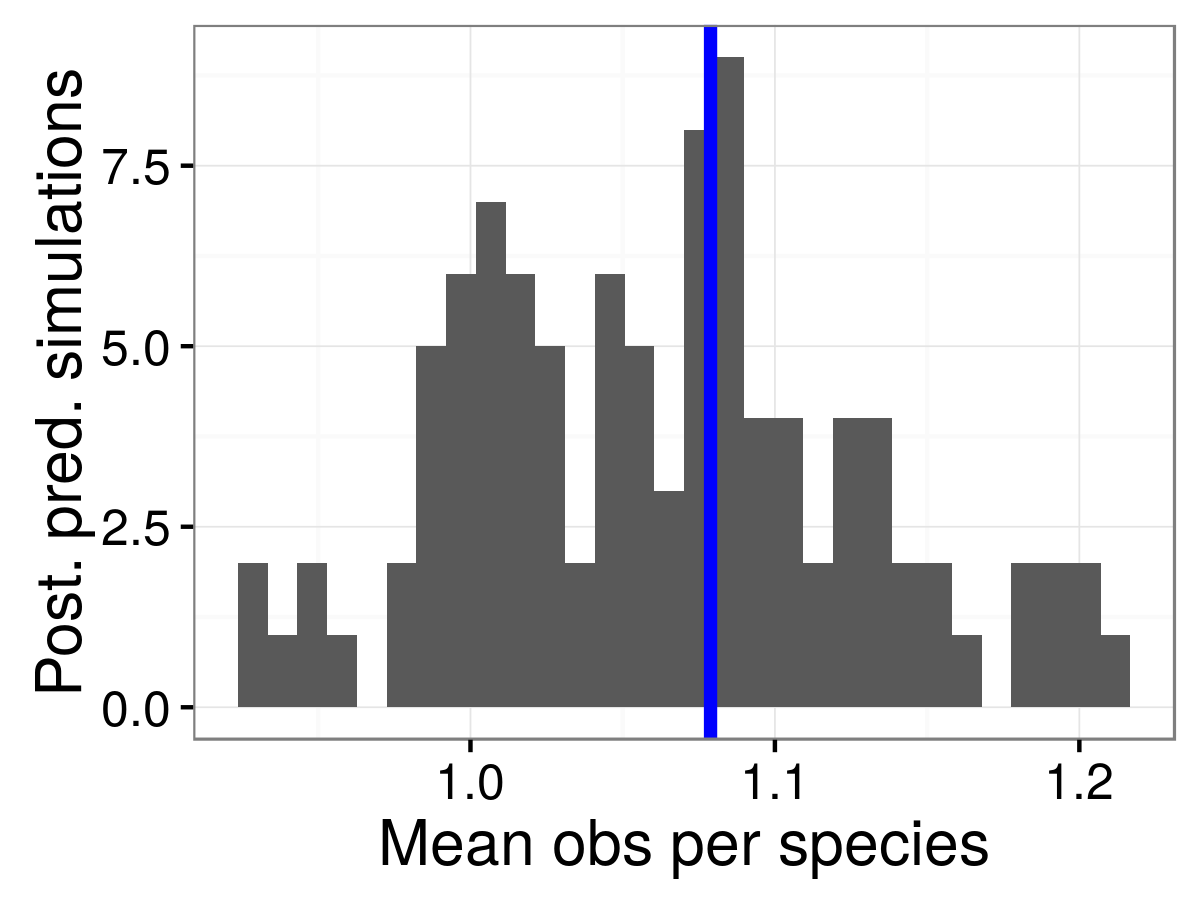
\includegraphics[width=\textwidth,height=0.3\textheight,keepaspectratio=true]{figure/pred_occ_bd}
  \caption[Posterior predictive check of average occurrence]{Comparison of the average observed number of occurrences per species (blue line) to the average number of occurrences from 100 posterior predictive datasets simulated from draws from the posterior parameter estimates from the model used in this study. The model is considered to have adequate fit to this aspect of the data if the observed value of the test statistic is approximately centered in the simulated distribution of test statistic values.}
  \label{fig:ppc}
\end{figure}


% observation process
%   time
Log-odds of observing a species given that it is present varies greatly with time (Fig. \ref{fig:time_observe}) with lowest log-odds of observation being during the Gerigian and Harrisonian land-mammal ages. It is important to note, however, that all land-mammal ages with log-odds of observation greater than 2 correspond to high probabilities of observation, which means that while there may be large differences in log-odds of observation between land-mammal ages this may not translate to substantial difference in the probability of observation. In particular, we might expect near perfect observation for most NALMA except for the Geringan, Harrisonian, Hemingfordian, and Clarendonian; this is not to say that the fossil record is complete, but that of those species observed there is little evidence supporting range extensions to species durations except the case of species that exist during or adjacent to these few NALMA. 
\begin{figure}[ht]
  \centering
  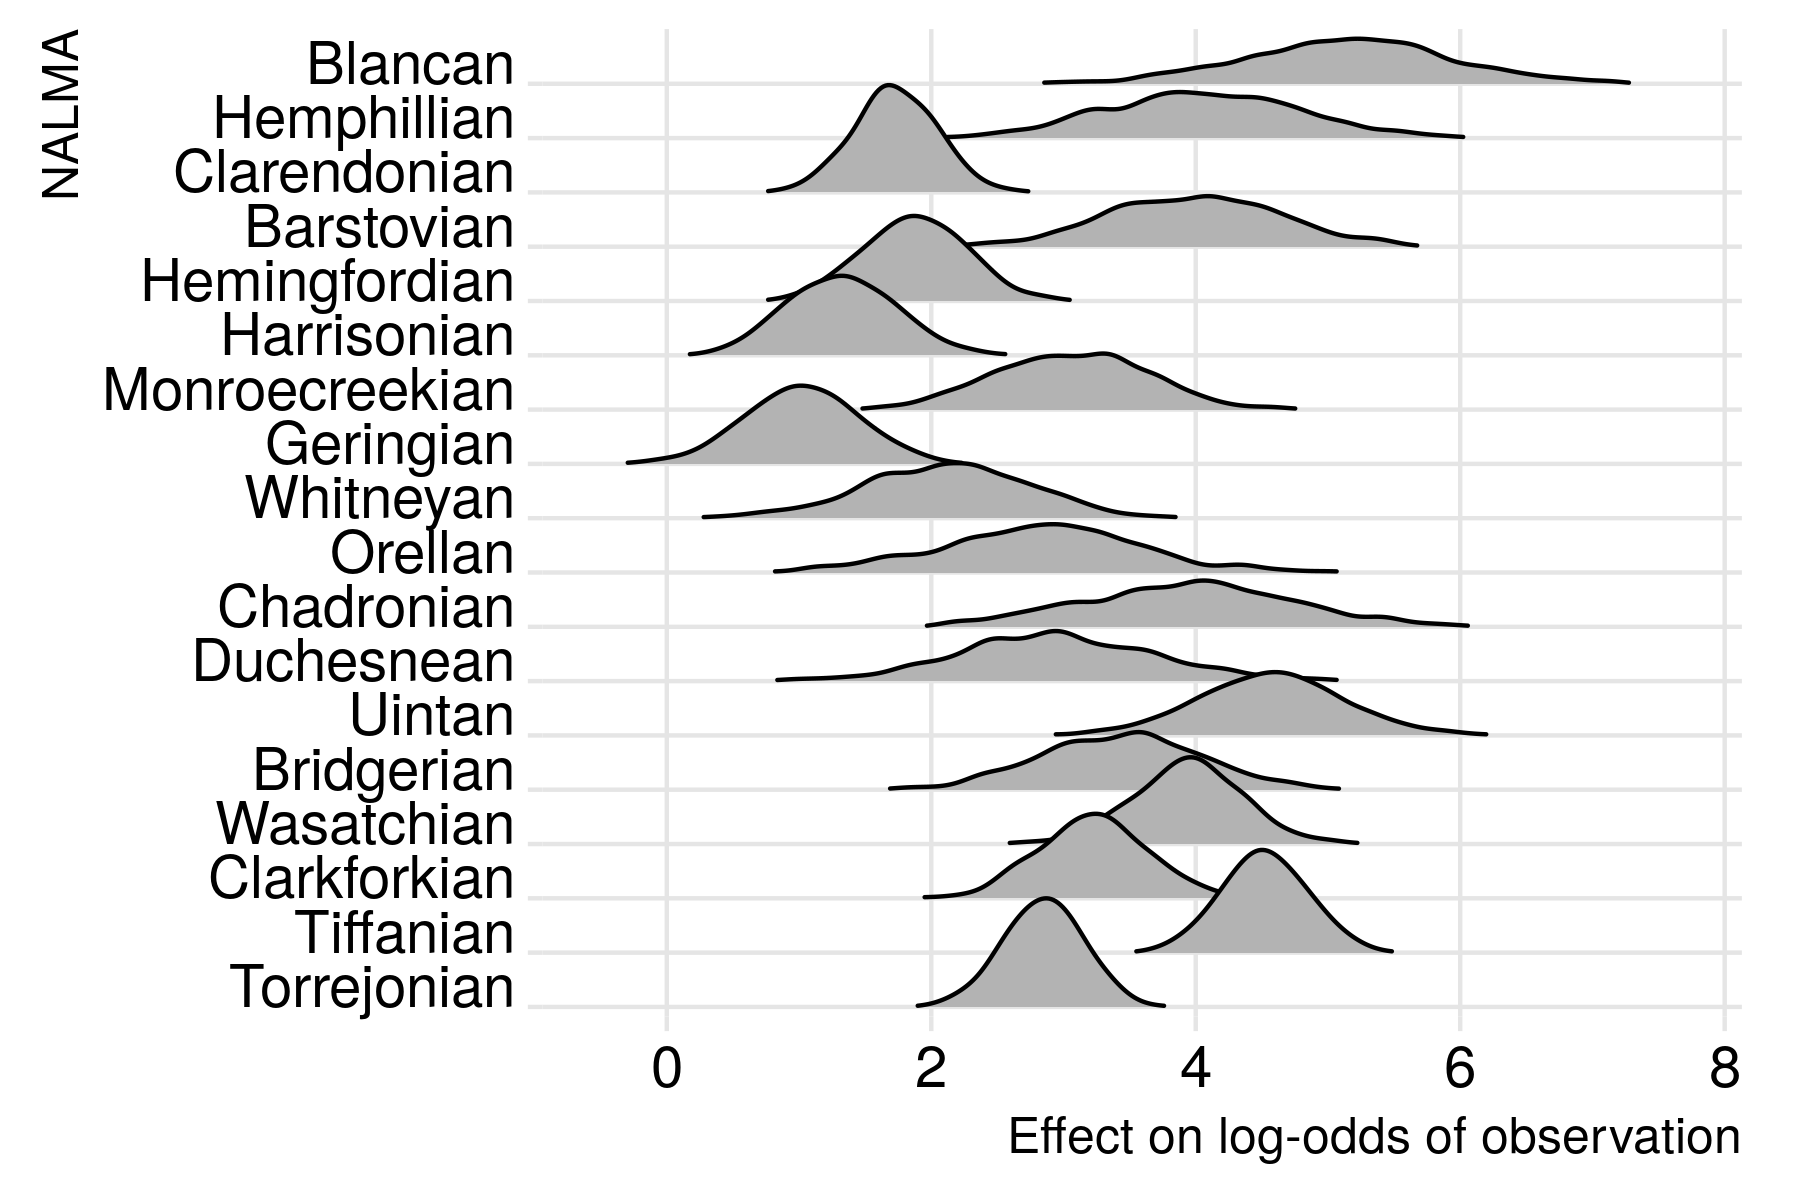
\includegraphics[width=\textwidth,height=0.4\textheight,keepaspectratio=true]{figure/time_observation}
  \caption{Ridgeline density plots of the estimates for the log-odds of observation from the time-varying intercept term. Each of the named time units are North American land-mammal ages. The oldest land-mammal age is at the bottom of the stack and the youngest is at the top. Higher values correspond to an greater log-odds of observation than lower values.}
  \label{fig:time_observe}
\end{figure}

%   functional group
In comparison to temporal variation, there is virtually no effect of functional group on the log-odds of observing a species that is present (Fig. \ref{fig:fg_observe}). All of the functional groups have approximately equal posterior distributions for their estimated effects on log-odds of observation, all of which are centered strongly on 0. These results not only indicate that observation is much more dependent on when the species occurs than the species ecology.
\begin{figure}[ht]
  \centering
  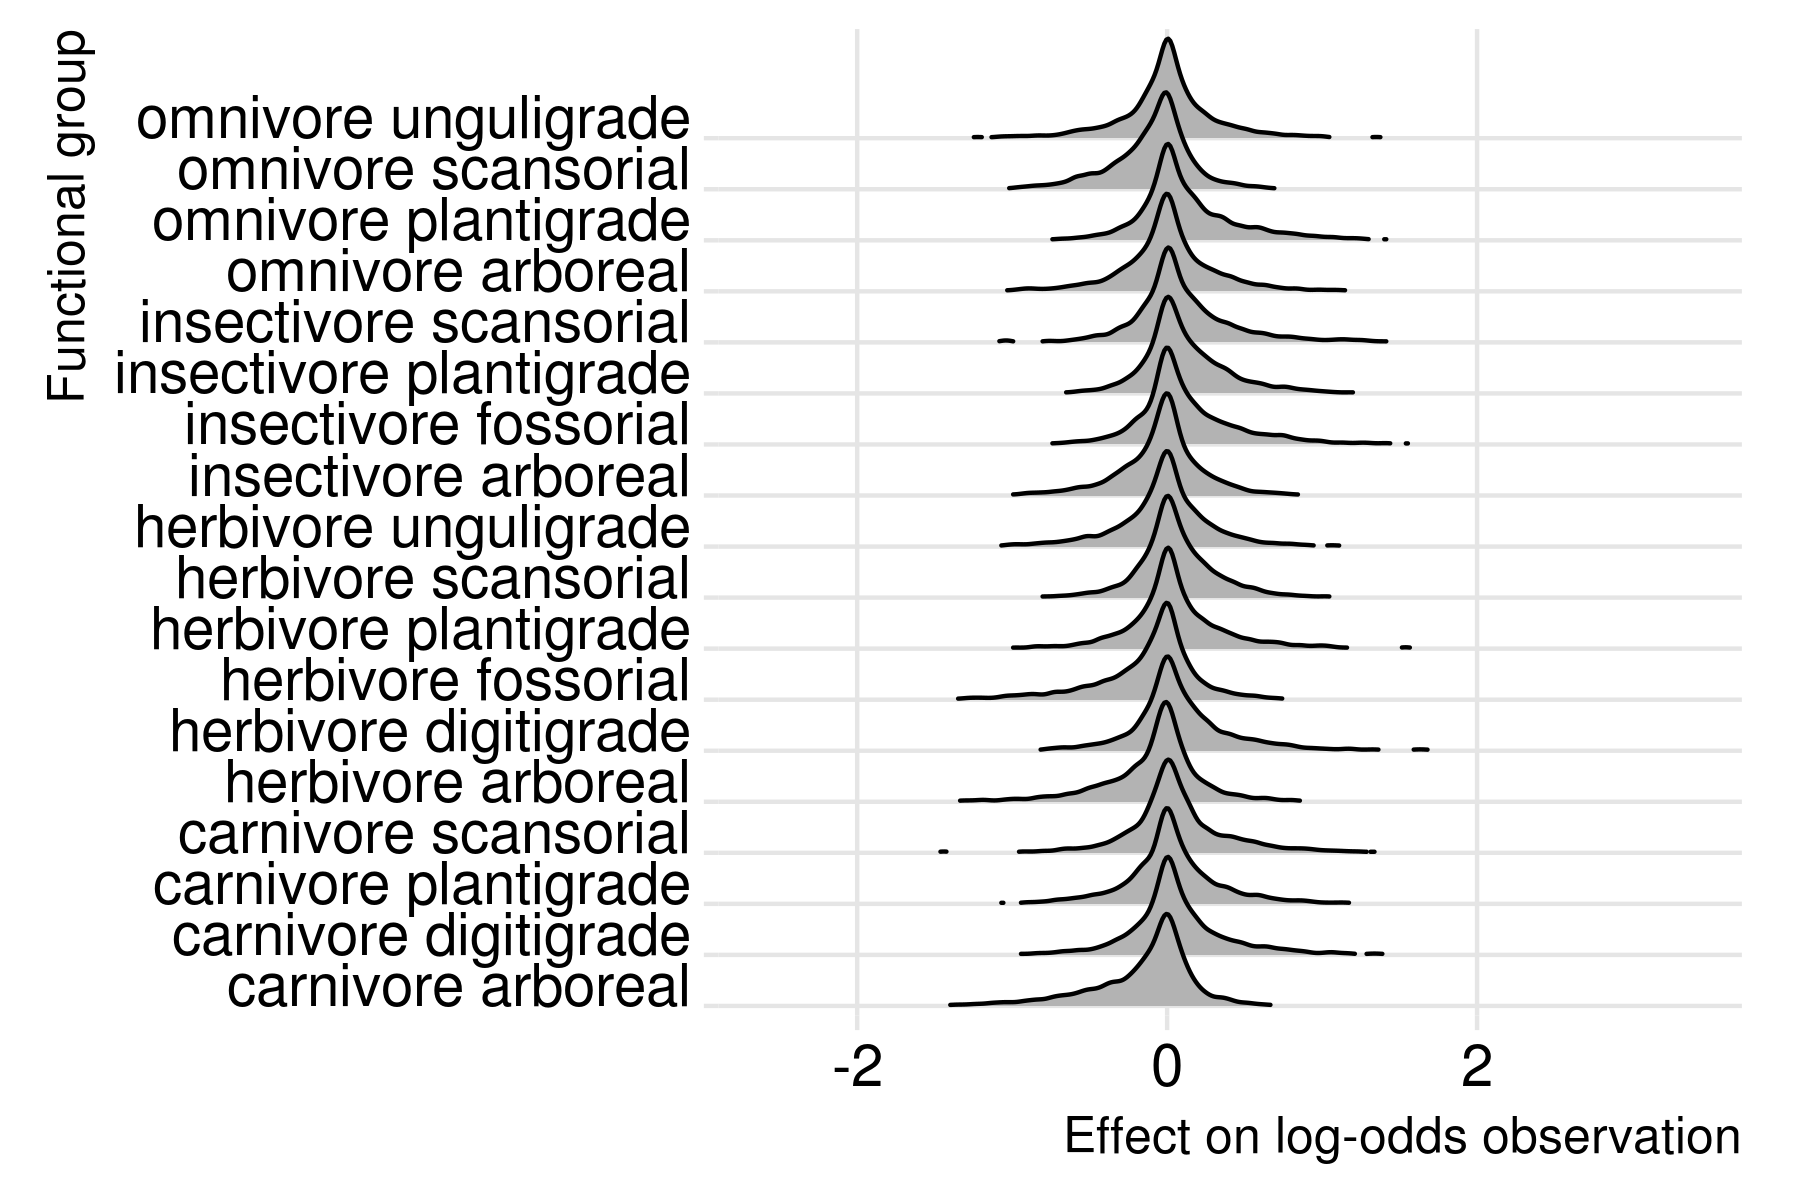
\includegraphics[width=\textwidth,height=0.4\textheight,keepaspectratio=true]{figure/ecotype_observation}
  \caption{Ridgeline density plots of the estimated effects of species' functional group on log-odds of observing that species given that it is present. Each of the rows correspond to a different functional group as indicated by the dietary and locomotor category combination. Positive values correspond to greater than average log-odds of observation, while negative values indicate lower than average log-odds of observation.}
  \label{fig:fg_observe}
\end{figure}

%   mass
Species mass is found to have a negative effect on observation probability, where species' with greater than average masses are estimated to not be observed as often as species with less than average species masses. The posterior probability of sign of this relationship is estimated to be 0.XX. However, this estimate does not necessarily translate to substantial differences in the estimated probability of observation because observation probability is so high for most of the Cenozoic (Fig. \ref{fig:time_observe}). In fact, it is only when observation probability is low that the effect of mass is easily observable. It is important to remember the effect of mass on observation was considered constant over time and that all differences observation probability between land-mammal ages is driven by variation over time. When log-odds of observation is high, differences due to covariate effects translate to very small differences in actual probability. While the coefficient describing the relationship between mass and observation is constant, the actual difference in terms of probability of observation can vary dramatically; for example, the Uintan and Geringian. 
\begin{figure}[ht]
  \centering
  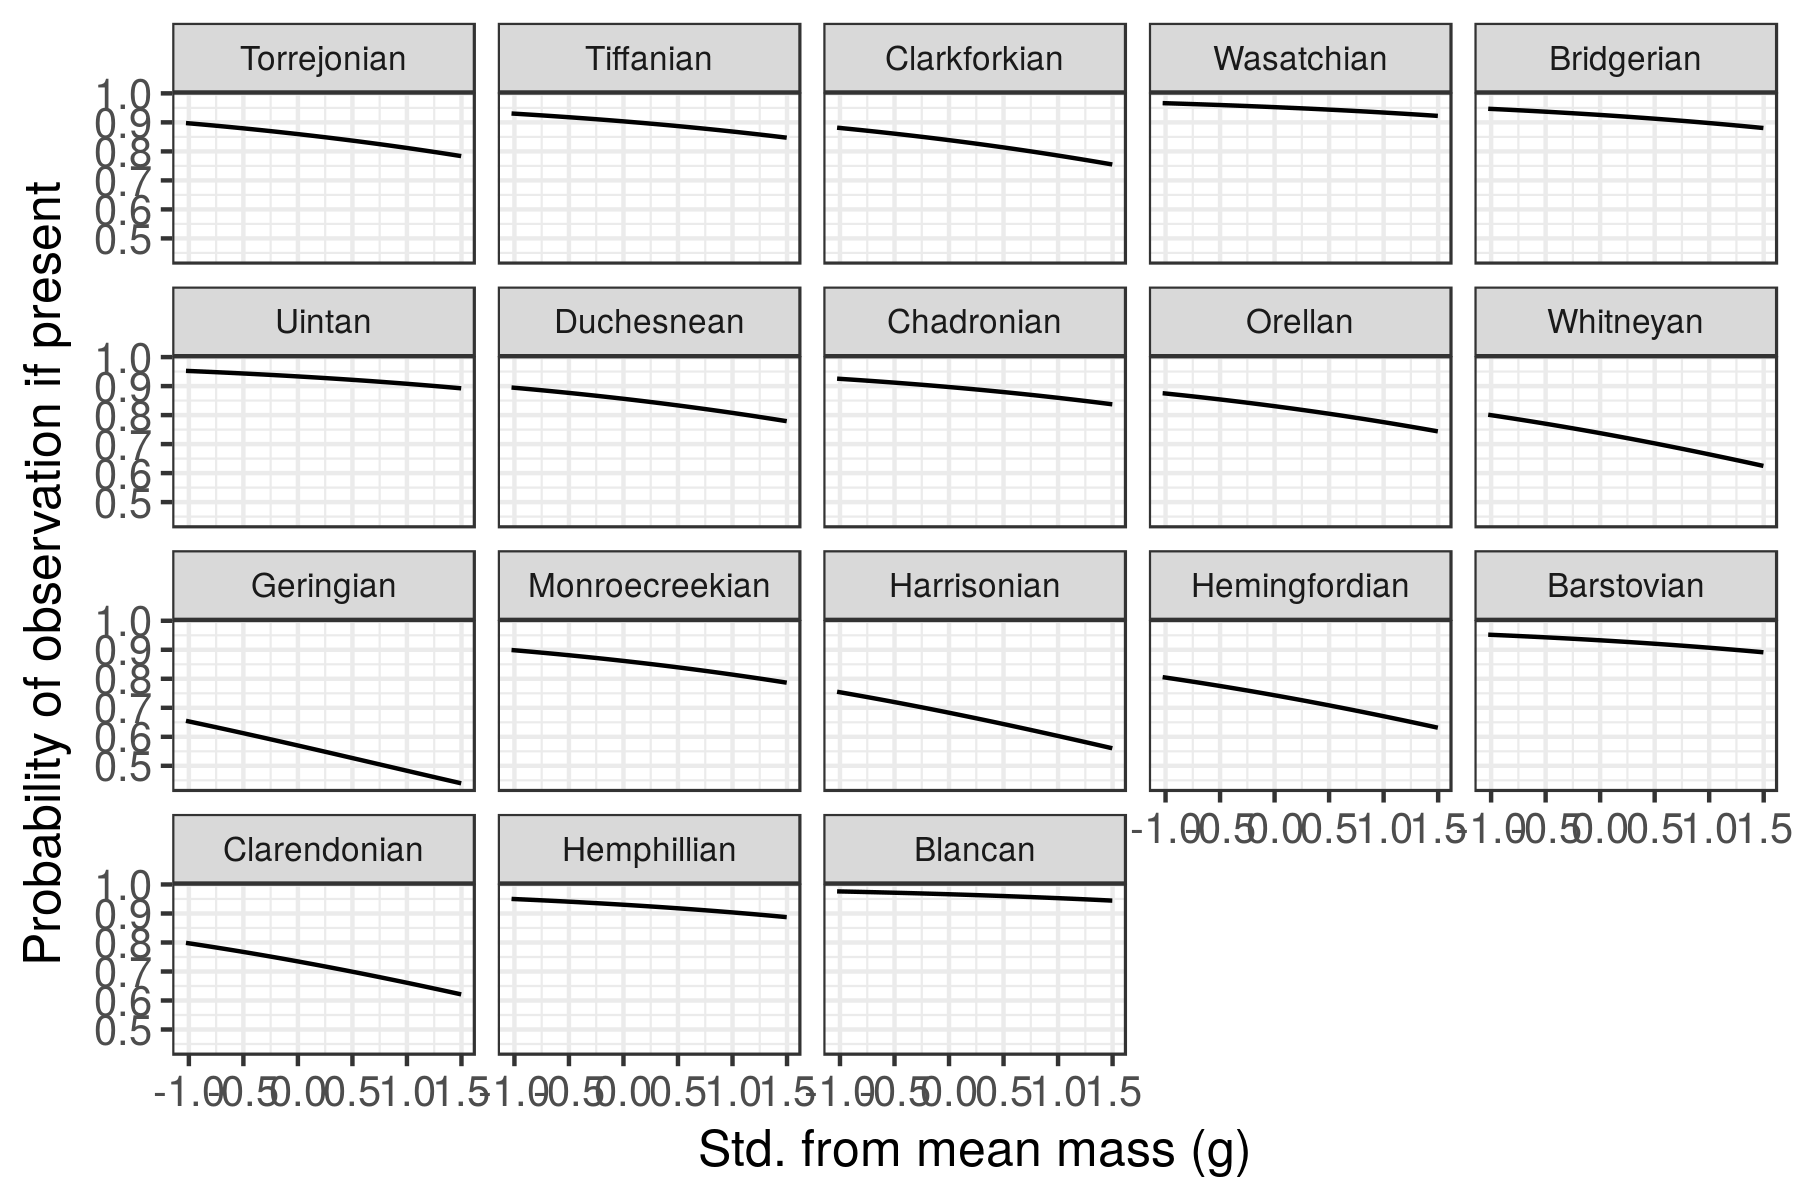
\includegraphics[width=\textwidth,height=0.4\textheight,keepaspectratio=true]{figure/mass_on_pres_bd}
  \caption[Estimates of the effect of mass on observation probability]{Estimates of the effect of species mass on probability of observing a species that is present (\(p\)). Mass has been log-transformed, centered, and rescaled; this means that a mass of 0 corresponds to the mean of log-mass of all observed species and that values are in units of standard deviations. The effect of mass on observation was considered constant over time, and variation in observation probability is due to the temporal effect (Fig. \ref{fig_observe}).} 
  \label{fig:mass_observe}
\end{figure}


% origination
%   individual-level
%     FG time series
Origination probability varies greatly among functional groups with each functional group exhibiting nearly unique time series with a few obviously shared features (Fig. \ref{fig:eco_origin}). When origination probability is below 0.50 this means that a new species of that functional group most likely will not enter the species pool, and when origination probability is greater than 0.50 then a new species of that functional group will probably entering the species pool. Finally, if origination probability is approximately 0.50, this indicates that it is equally likely that a new species will enter the species pool as it will not. The slope of origination probability time-series is also very revealing; when the slope of the time series is positive then new species are being added to the species pool, and when the slope is negative it is expected that the number of new species entering the pool is decreasing with time. %Importantly, large uncertainty in probabilities can reflect complete separation which results from that functional group leaving the species pool and therefore it's absence is without ambiguity CITATION. 

Most of the functional groups have origination probabilities of approximately 1 by the present (Fig. \ref{fig:eco_origin}); new species in these functional groups are being added to the species pool through out the Cenozoic. Additionally, this pattern reflects the increasing certainty of species which have no originated yet originating in the subsequent time step. If a functional group reaches origination probability of 1 before the present, then there is a high chance that all species of that functional group originated well before the present; this means that even if a group has origination probability 1, if there are no more species of that group which could have originated based on the observed species, then no new species will enter this system.

\uppercase{more}

\begin{figure}[ht]
  \centering
  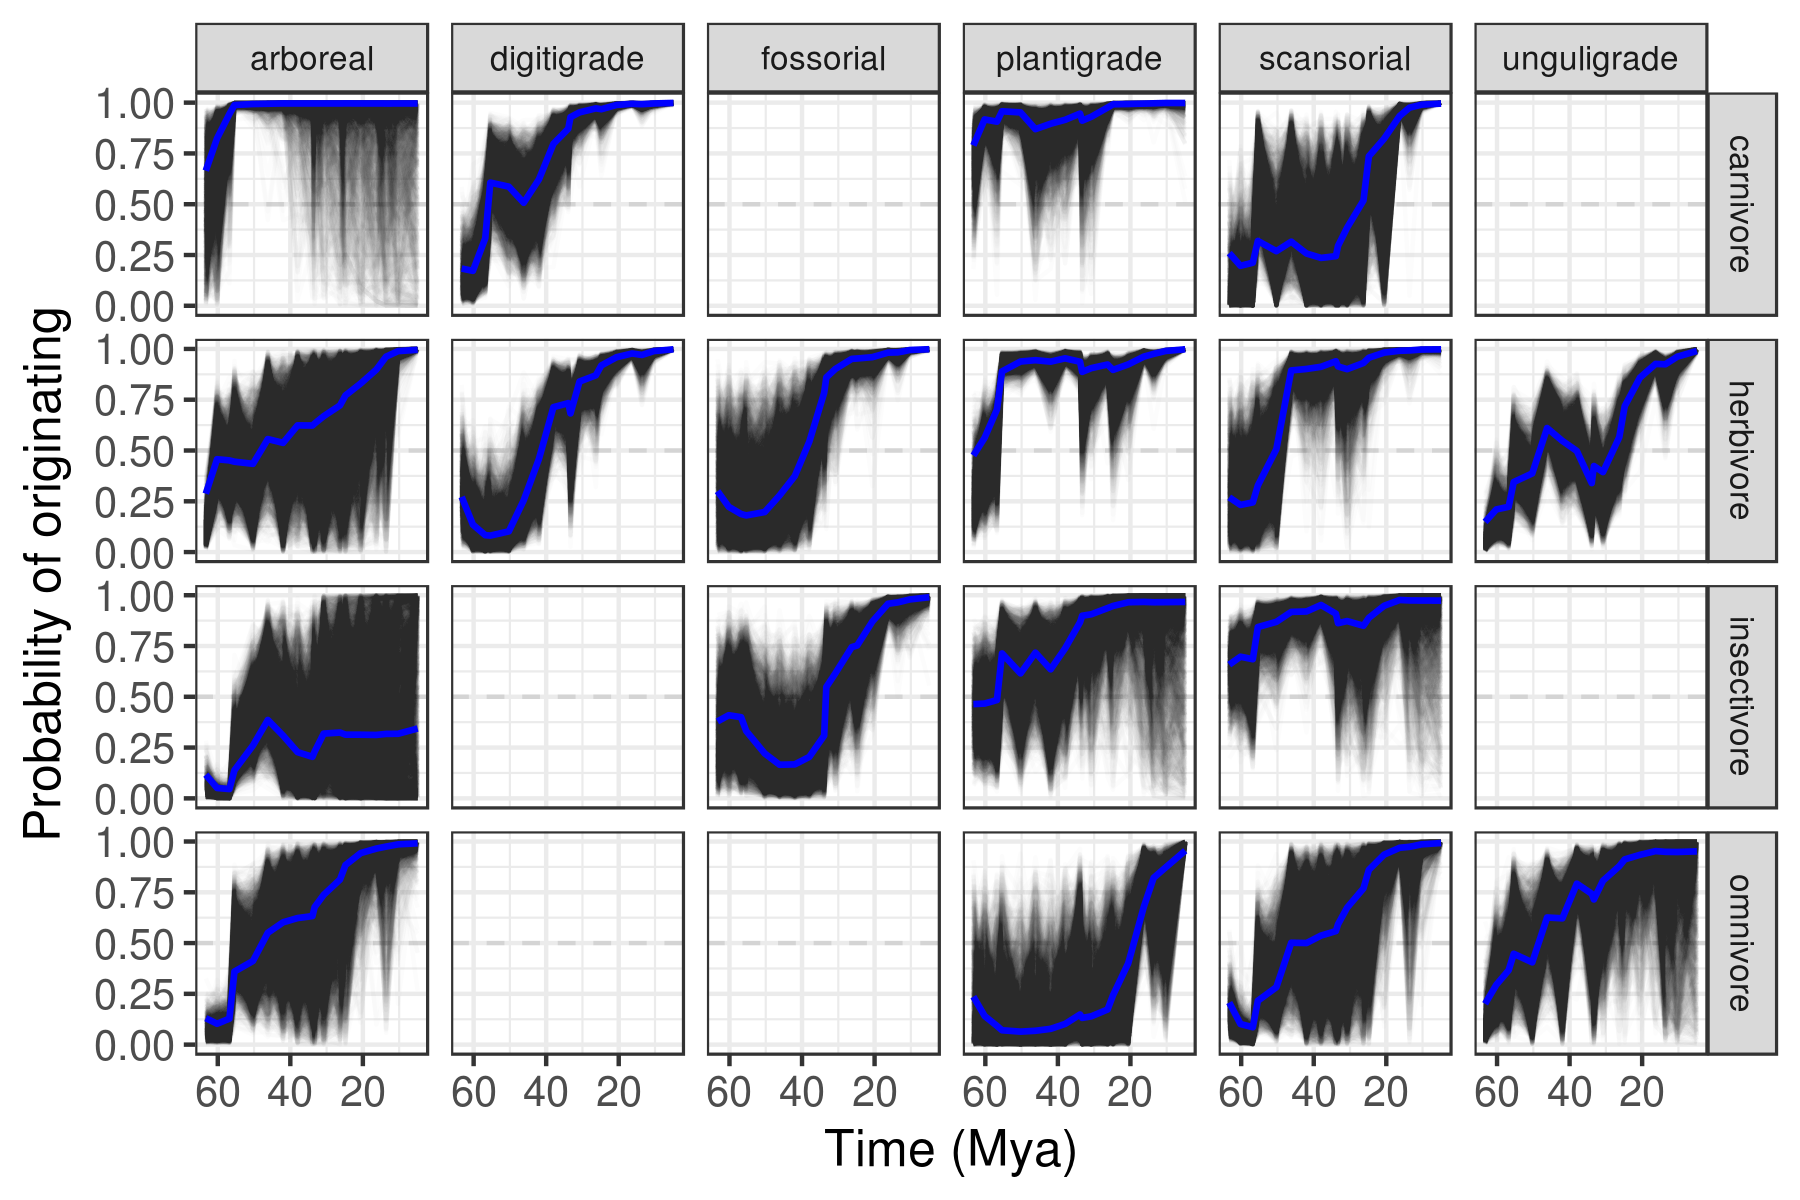
\includegraphics[width=\textwidth,height=0.4\textheight,keepaspectratio=true]{figure/ecotype_origin_bd}
  \caption{Probability of a species first originating based on functional group. Origination probability is graphed as 100 time-series drawn from the model's posterior estimates. A greater density of the posterior estimates indicates increased certainty. The blue line is the mean origination probability as predicted by just the group-level predictors. The columns are by locomotor category and rows by dietary category.}
  \label{fig:eco_origin}
\end{figure}

%     order effect
Origination probability varies greatly amongst mammal orders (Fig. \ref{fig:order_origin}). These estimates reflect differences origination probability as well as the relative rarity of that order in the fossil record; if there are few members of that order and they are distributed through time then they would have an inherently lower probability of origination. Orders with greater than average log-odds of origination include Condylarthra, Dinocerata, Multituverculata, and Primates; orders that have considered important components of the Paleogene fossil record. Orders with lower than average log-odds of origination include Acreodi, Artiodactyla, Carnivora, Cimolesta, Cingulata, Eulipotyphla, Lagomorpha, Leptictida, Macroscelidea, Perissodactyla, Pholidota, Pilosa, Proboscidea, Rodentia; orders characterized by either small body size or primarily Neogene records. Additionally, the variance between orders is vary large ranging from -5 to 3 log-odds of origination; this large of variance reflects how species within these orders have very different patterns of origination independent from their origination based on functional ecology (Fig. \ref{fig:eco_origin}).
\begin{figure}[ht]
  \centering
  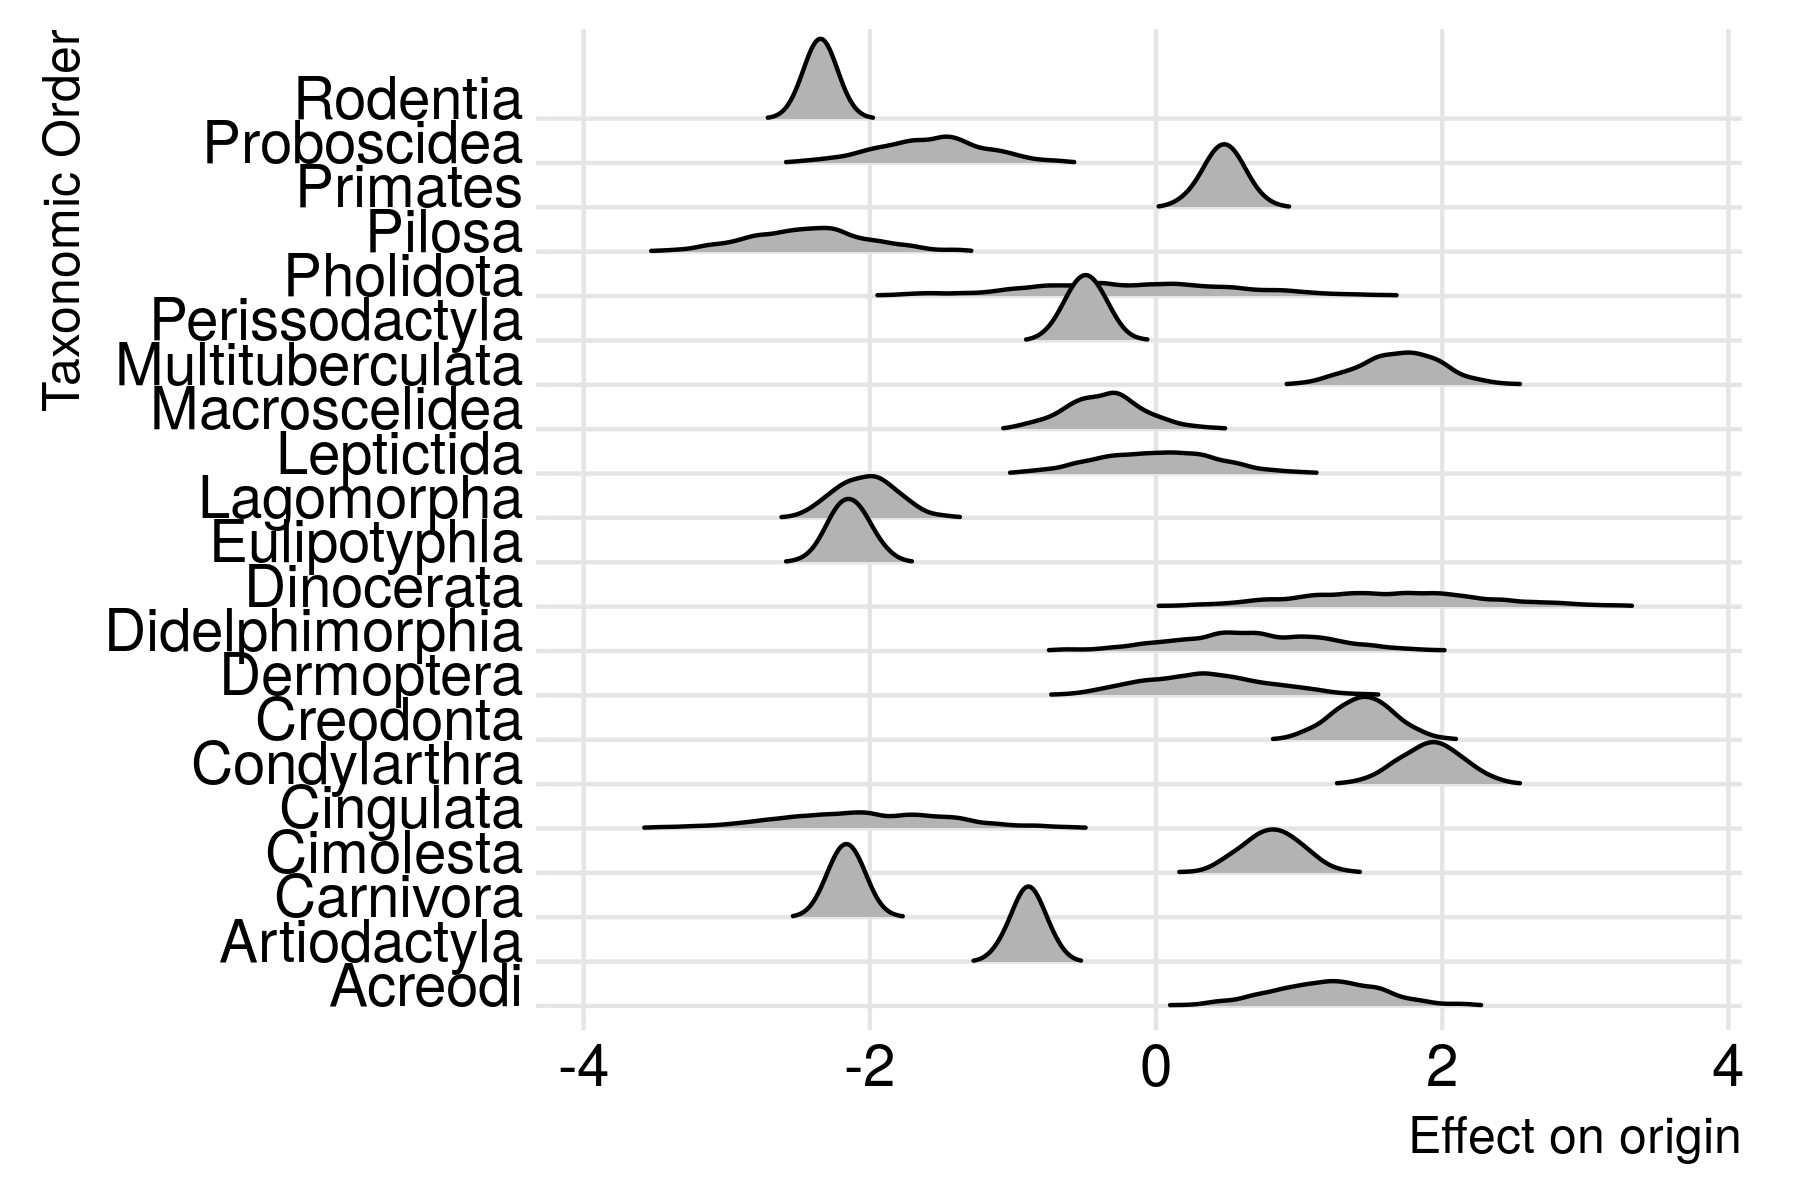
\includegraphics[width=\textwidth,height=0.4\textheight,keepaspectratio=true]{figure/order_origin_bd}
  \caption{Ridgeline density plots of estimated log-odds of origination based on mammal orders. Positive values correspond to greater log-odds origination than average, while negative values correspond to lower log-odds of origination than average. Importantly, origination probability corresponds to the rarity of that order in the fossil record as well as differences in origination due to species' order (rare orders have few originations)}
  \label{fig:order_origin}
\end{figure}

%     mass effect
Species mass is estimated to have a negative relationship with origination probability (P(\(\beta^{\phi} < 0\)) = 1; Fig. \ref{fig:mass_origin}) meaning that species with greater than average mass have a lower probability of originating at any point in time than species with below average mass. This result is sensible given the left-skewed distribution of mammal species body sizes where large body sizes form the right-hand tail. There are fewer large body-sized mammals which have ever originated than small body sized mammals. Interestingly, many of the orders with small body sizes (e.g. Rodentia, Lagomorpha) have below average origination probabilities (Fig. \ref{fig:order_origin}); when this result is considered together with the effect of mass on origination these effects could be counteracting each other. These results continue to add to the understanding of the heterogeneity and nuance associated with species origination dynamics.
\begin{figure}[ht]
  \centering
  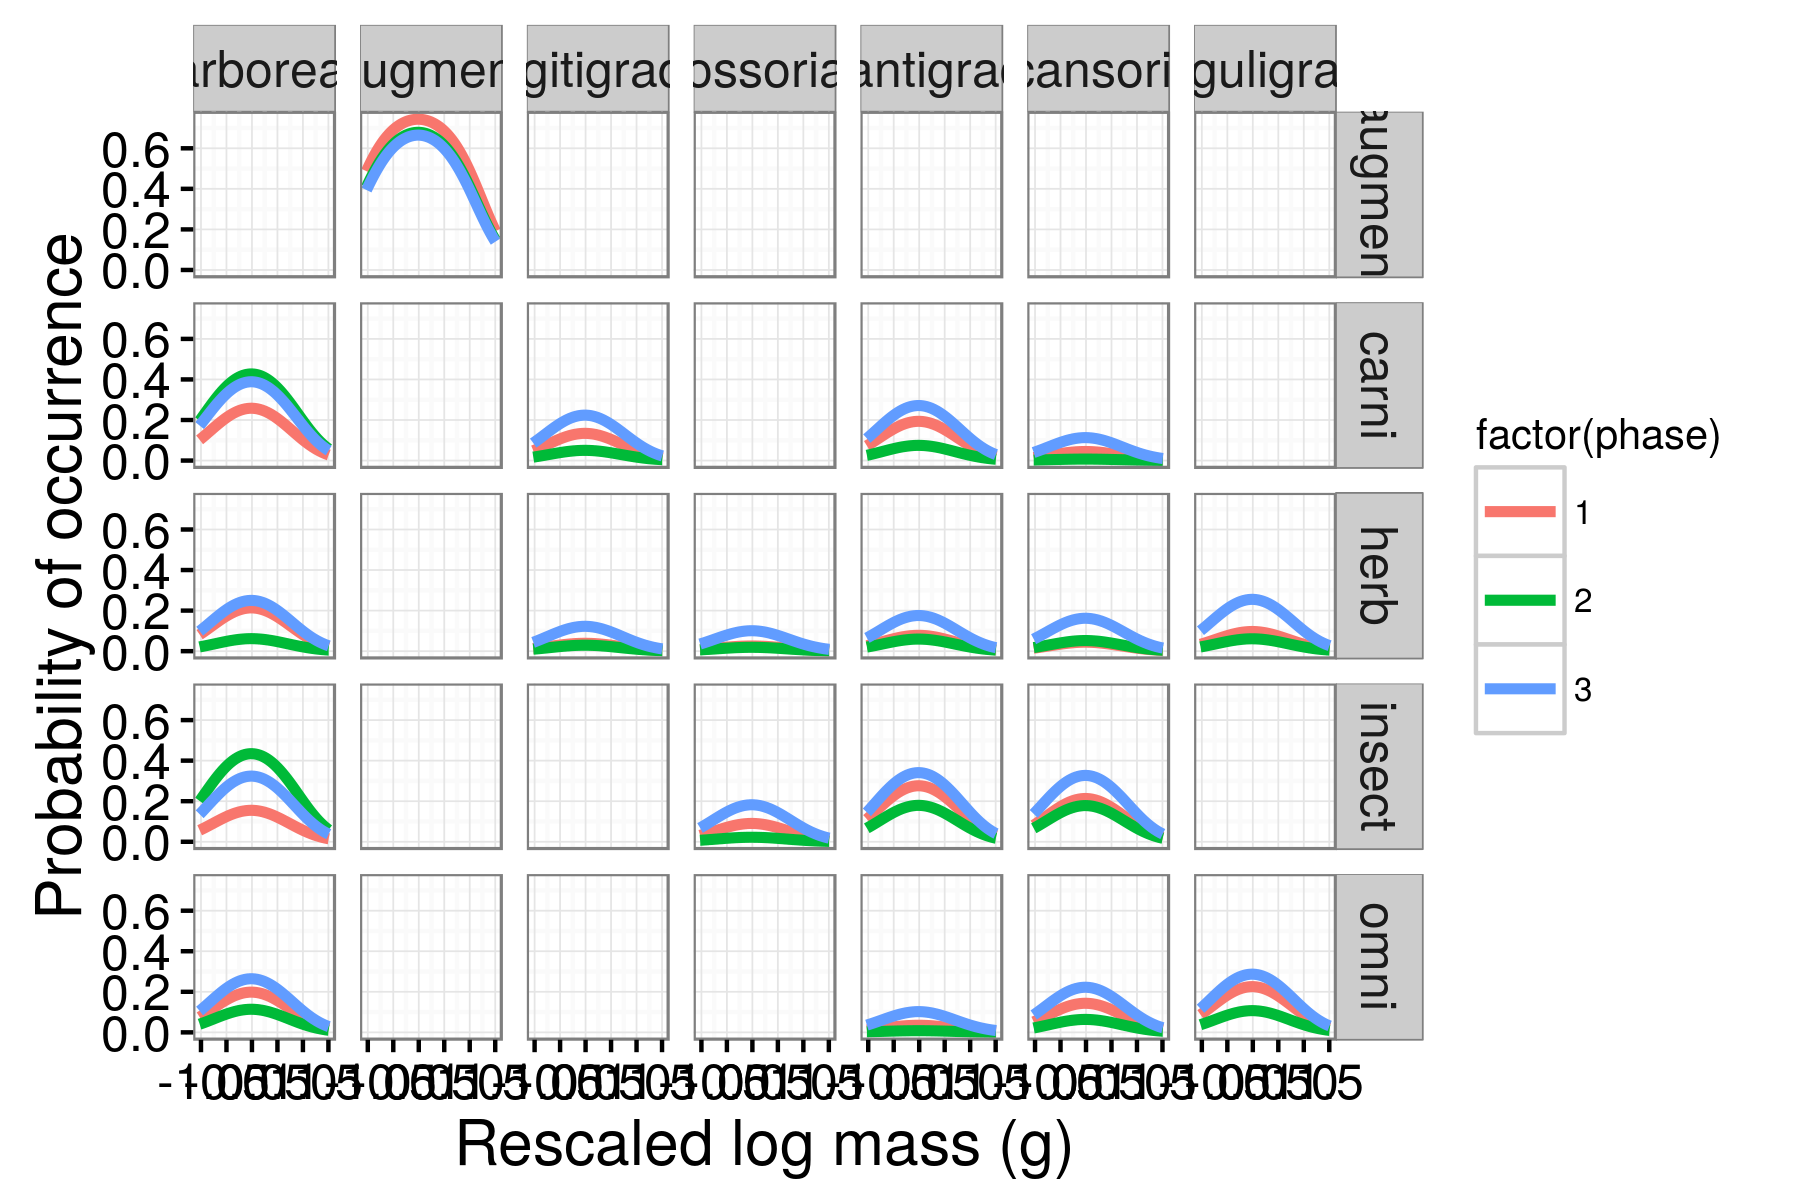
\includegraphics[width=\textwidth,height=0.4\textheight,keepaspectratio=true]{figure/mass_on_origin_bd}
  \caption{Mean estimates of the effect of species' mass on the probability of a species originating, plotted for each of the three plant phases. While the effect of mass is considered constant over time, each plant phases corresponds to a different intercept of the relationship between mass and origination. The three plant phases are indicated by the color of the line. Mass has been log-transformed, centered, and rescaled; this means that a mass of 0 corresponds to the mean of log-mass of all observed species and that mass is in standard deviation units. For clarity, only the mean of these estimates is plotted.}
  \label{fig:mass_origin}
\end{figure}

%   group-level
%     temperature and plant phase
For most functional groups, origination probabilities are not estimated to be distinct by plant phase (Fig. \ref{fig:group_origin_bd}, Table \ref{tab:origin_plant}). Additionally, there is no evidence that global temperature is a good predictor of origination probability, positive or negative (Fig. \ref{fig:group_origin_bd}, Table \ref{tab:origin_temp}).

There are no examples of functional groups having a difference in origination probability between the Eocene-Miocene and Miocene-Pliocene plant phases (Table \ref{tab:origin_plant}). There is weak evidence (P\(>\)0.8) that scansorial herbivores and unguligrade herbivores have greater origination probabilities during the Miocene-Pliocene than the Paleocene-Eocene (Table \ref{tab:origin_plant}). Finally, there is weak evidence (P\(>\)0.8) that plantigrade carnivores have greater origination probability during the Paleocene-Eocene than the Eocene-Miocene; in contrast, there is weak evidence that plantigrade carnivores have greater origination probability during the Eocene-Miocene than the Paleocene-Eocene (Table \ref{tab:origin_plant}).
\begin{figure}[ht]
  \centering
  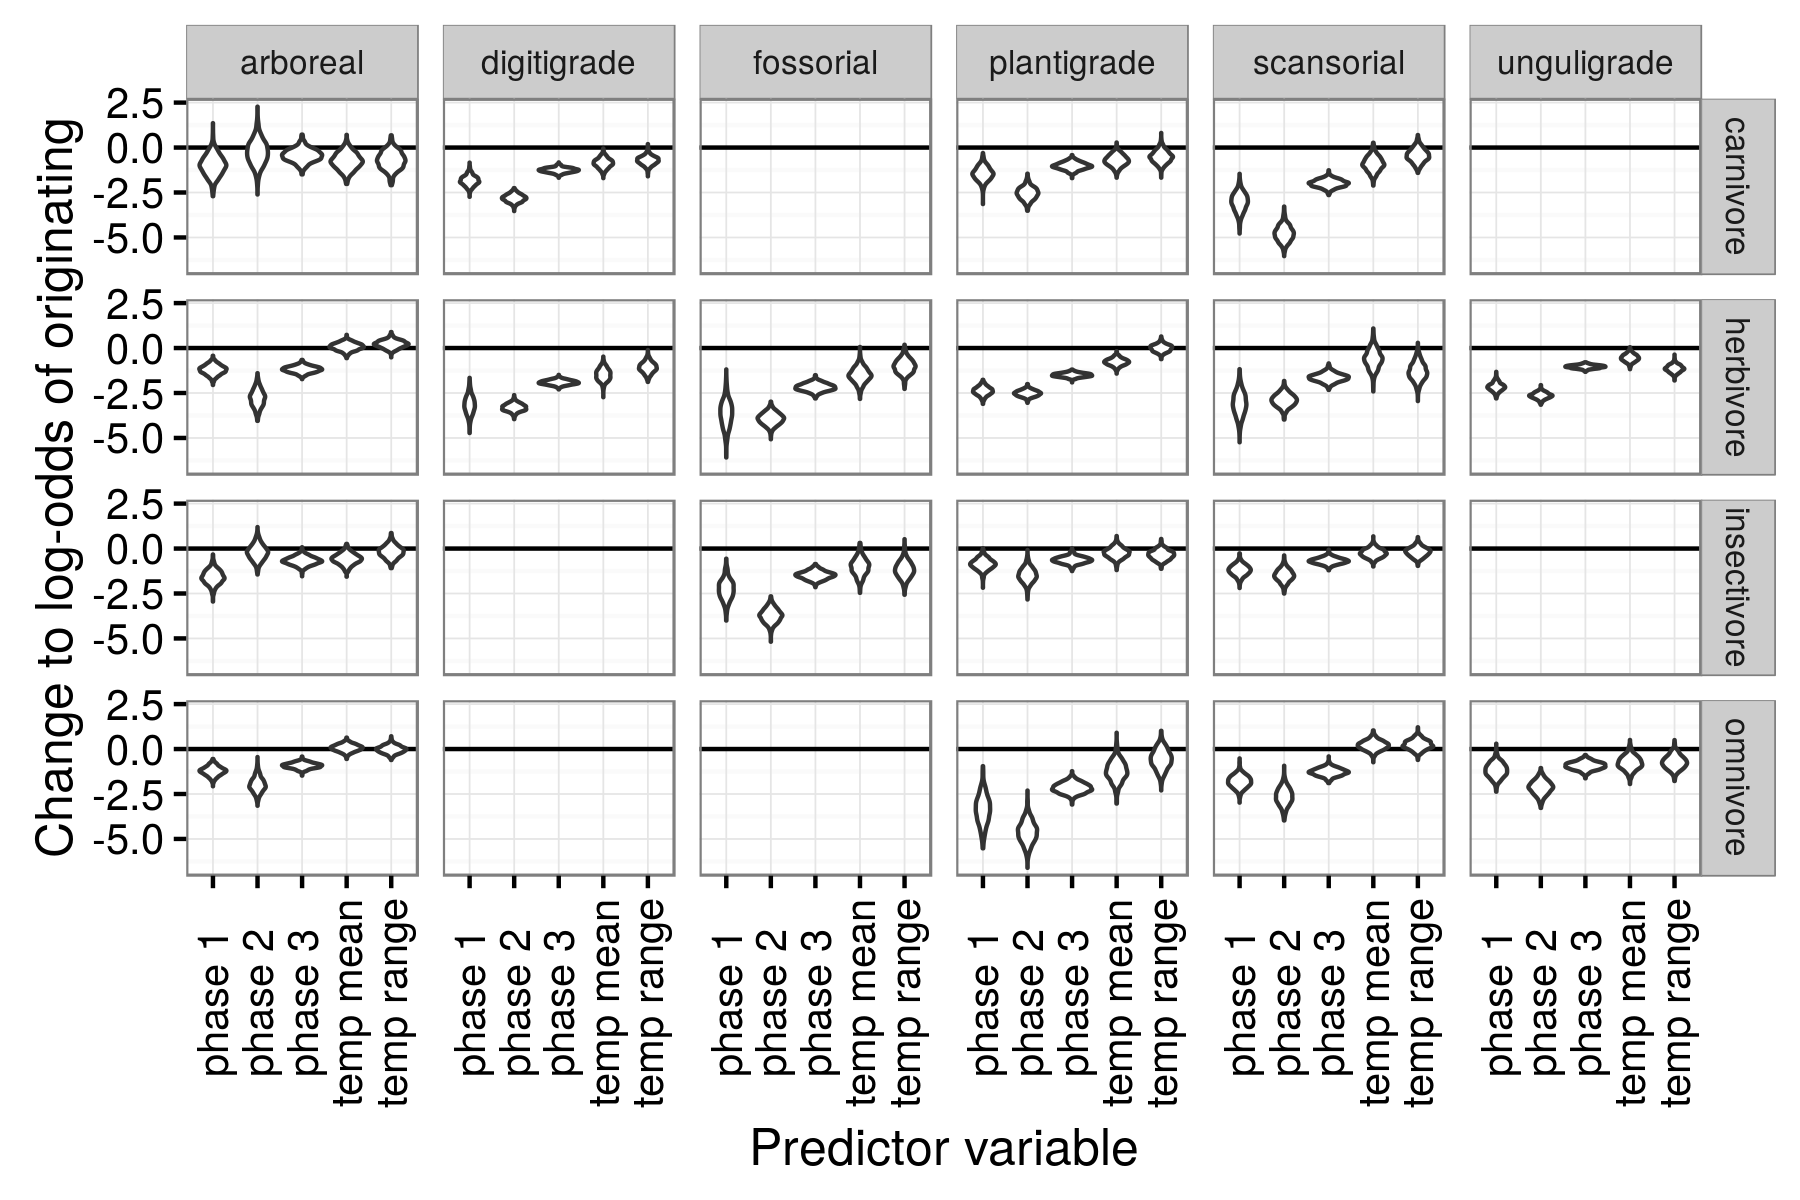
\includegraphics[width=\textwidth,height=0.4\textheight,keepaspectratio=true]{figure/group_on_origin_bd}
  \caption{Estimated effects of the group-level covariates describing environmental context on log-odds of species origination. The violin densities that are plotted are based on 1000 samples from the approximate posterior. The color of the violin corresponds to the probability that the covariates effect is estimated to be greater than 0; red values correspond to greater than 0.50 probability of being positive, blue values correspond to less than 0.50 probability of being positive.} 
  \label{fig:group_origin_bd}
\end{figure}

% make these tables appendix
\begin{table}[ht]
  \centering
  \caption[Posterior probablity estimates of differences in origination by plant phase]{Probability of a plant phase having greater log-odds of originating than another. The first two columns are comparisons of that posterior estimate to zero, which corresponds to the probability of that plant phase having a greater log-odds of originating when compared to the Miocene-Pleistocene. The final columnn corresponds to the comparison in log-odds of originating between the Eocene-Miocene and the Paleocene-Eocene.} 
  \label{tab:origin_plant}
  \begin{tabular}{ l r r r }
    \hline
    & P(Eo.Mi $>$ 0) & P(Pa.Eo $>$ 0) & P(Eo.Mi $>$ Pa.Eo) \\ 
    \hline
    arboreal carnivore & 0.555 & 0.577 & 0.489 \\ 
    digitigrade carnivore & 0.470 & 0.385 & 0.568 \\ 
    plantigrade carnivore & 0.359 & 0.787 & 0.196 \\ 
    scansorial carnivore & 0.370 & 0.339 & 0.536 \\ 
    arboreal herbivore & 0.396 & 0.316 & 0.562 \\ 
    digitigrade herbivore & 0.645 & 0.276 & 0.760 \\ 
    fossorial herbivore & 0.527 & 0.359 & 0.624 \\ 
    plantigrade herbivore & 0.446 & 0.509 & 0.461 \\ 
    scansorial herbivore & 0.698 & 0.179 & 0.851 \\ 
    unguligrade herbivore & 0.580 & 0.196 & 0.778 \\ 
    arboreal insectivore & 0.529 & 0.213 & 0.735 \\ 
    fossorial insectivore & 0.429 & 0.469 & 0.475 \\ 
    plantigrade insectivore & 0.556 & 0.433 & 0.597 \\ 
    scansorial insectivore & 0.601 & 0.543 & 0.548 \\ 
    arboreal omnivore & 0.484 & 0.221 & 0.699 \\ 
    plantigrade omnivore & 0.386 & 0.341 & 0.533 \\ 
    scansorial omnivore & 0.549 & 0.242 & 0.731 \\ 
    unguligrade omnivore & 0.587 & 0.255 & 0.731 \\ 
    \hline
  \end{tabular}
\end{table}

\begin{table}[ht]
  \centering
  \caption[Posterior probablity of effects of temperature on origination]{Probability that the two temperature covariates have an effect on the log-odds of functional group origination. Values greater than 0.50 correspond to the probability of that effect having positive relationship with origination, while values less than 0.5 correspond increasing certainty that that covariate has a negative relationship with origination.}
  \label{tab:origin_temp}
  \begin{tabular}{ l r }
    \hline
    & \(P(\gamma_{temp\ mean} > 0)\) \\
    \hline
    arboreal carnivore & 0.492 \\ 
    digitigrade carnivore & 0.256 \\ 
    plantigrade carnivore & 0.611 \\ 
    scansorial carnivore & 0.334 \\ 
    arboreal herbivore & 0.353 \\ 
    digitigrade herbivore & 0.240 \\ 
    fossorial herbivore & 0.320 \\ 
    plantigrade herbivore & 0.323 \\ 
    scansorial herbivore & 0.322 \\ 
    unguligrade herbivore & 0.291 \\ 
    arboreal insectivore & 0.223 \\ 
    fossorial insectivore & 0.448 \\ 
    plantigrade insectivore & 0.440 \\ 
    scansorial insectivore & 0.464 \\ 
    arboreal omnivore & 0.232 \\ 
    plantigrade omnivore & 0.314 \\ 
    scansorial omnivore & 0.270 \\ 
    unguligrade omnivore & 0.313 \\ 
    \hline
  \end{tabular}
\end{table}

%     correlation
The origination probabilities of four mammal functional groups are estimated with weak support (P\(>\)0.8) to be positively correlated (Fig. \ref{fig:origin_sig_corr}); importantly, because of the random-walk prior on the intercepts of the group-level regressions, these correlations specifically reflect similarities in origination probability time series beyond their intrinsic temporal autocorrelation. These correlations give a weak indication that the probability that species of the correlated functional groups are entering the system rise and fall at similar times. Plantigrade herbivores, unguligrade herbivores, and scansorial herbivores are all found with weak evidence of being cross-correlated. Similarly, plantigrade omnivores are estimated to have correlated origination probabilities with just plantigrade herbivores and scansorial carnivores. 
%\begin{figure}[ht]
%  \centering
%  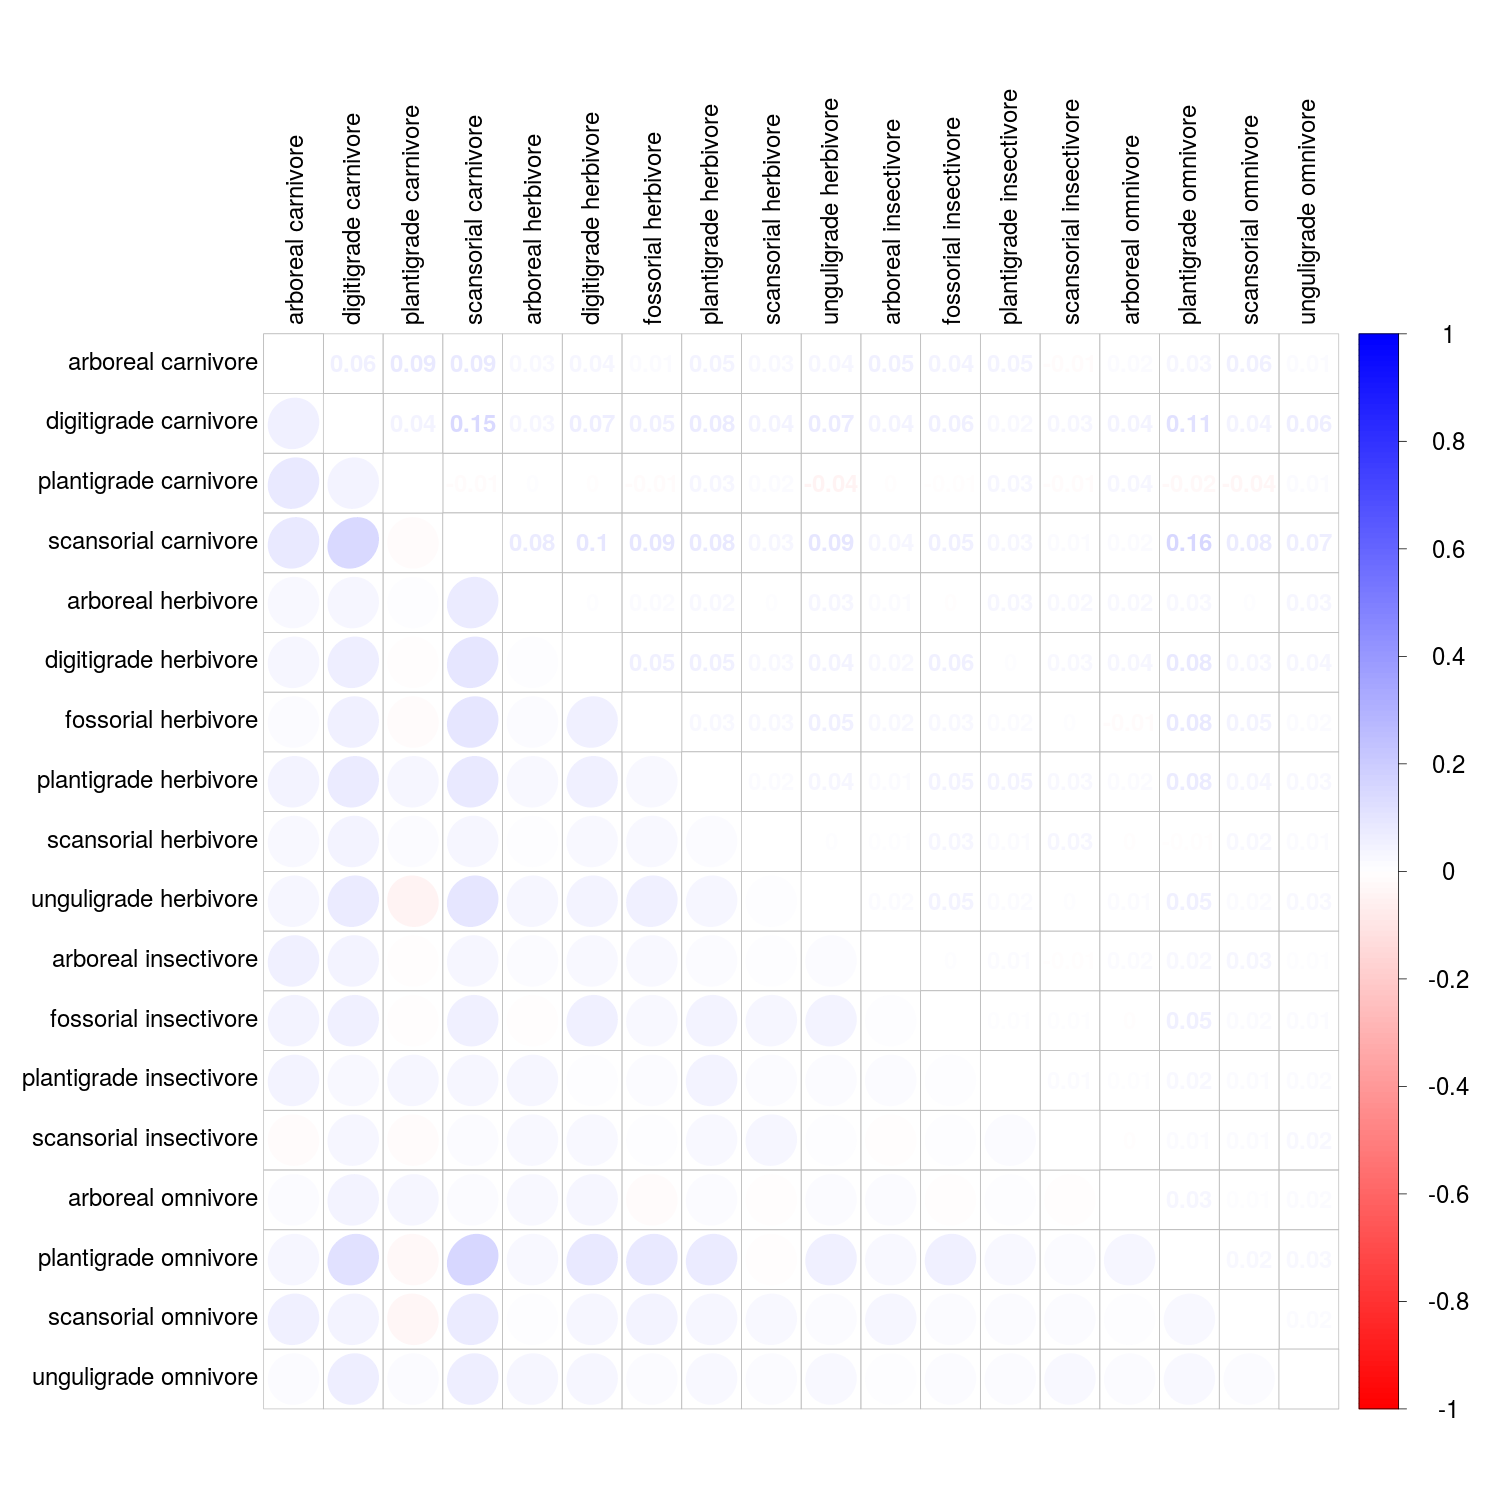
\includegraphics[width=\textwidth,height=\textheight,keepaspectratio=true]{figure/origination_correlation}
%  \caption{Posterior estimate of mean correlations in origination probability between the mammal functional groups. The lower triangle of the matrix is populated with ellipses corresponding to the level of correlation between the two functional groups, while the upper triangle of the matrix corresponds to the mean estimate of the correlation between functional groups. Darker values correspond to a greater magnitude of correlation with blue values corresponding to a positive correlation and red values a negative correlation.}
%  \label{fig:origin_corr}
%\end{figure}
%
\begin{figure}[ht]
  \centering
  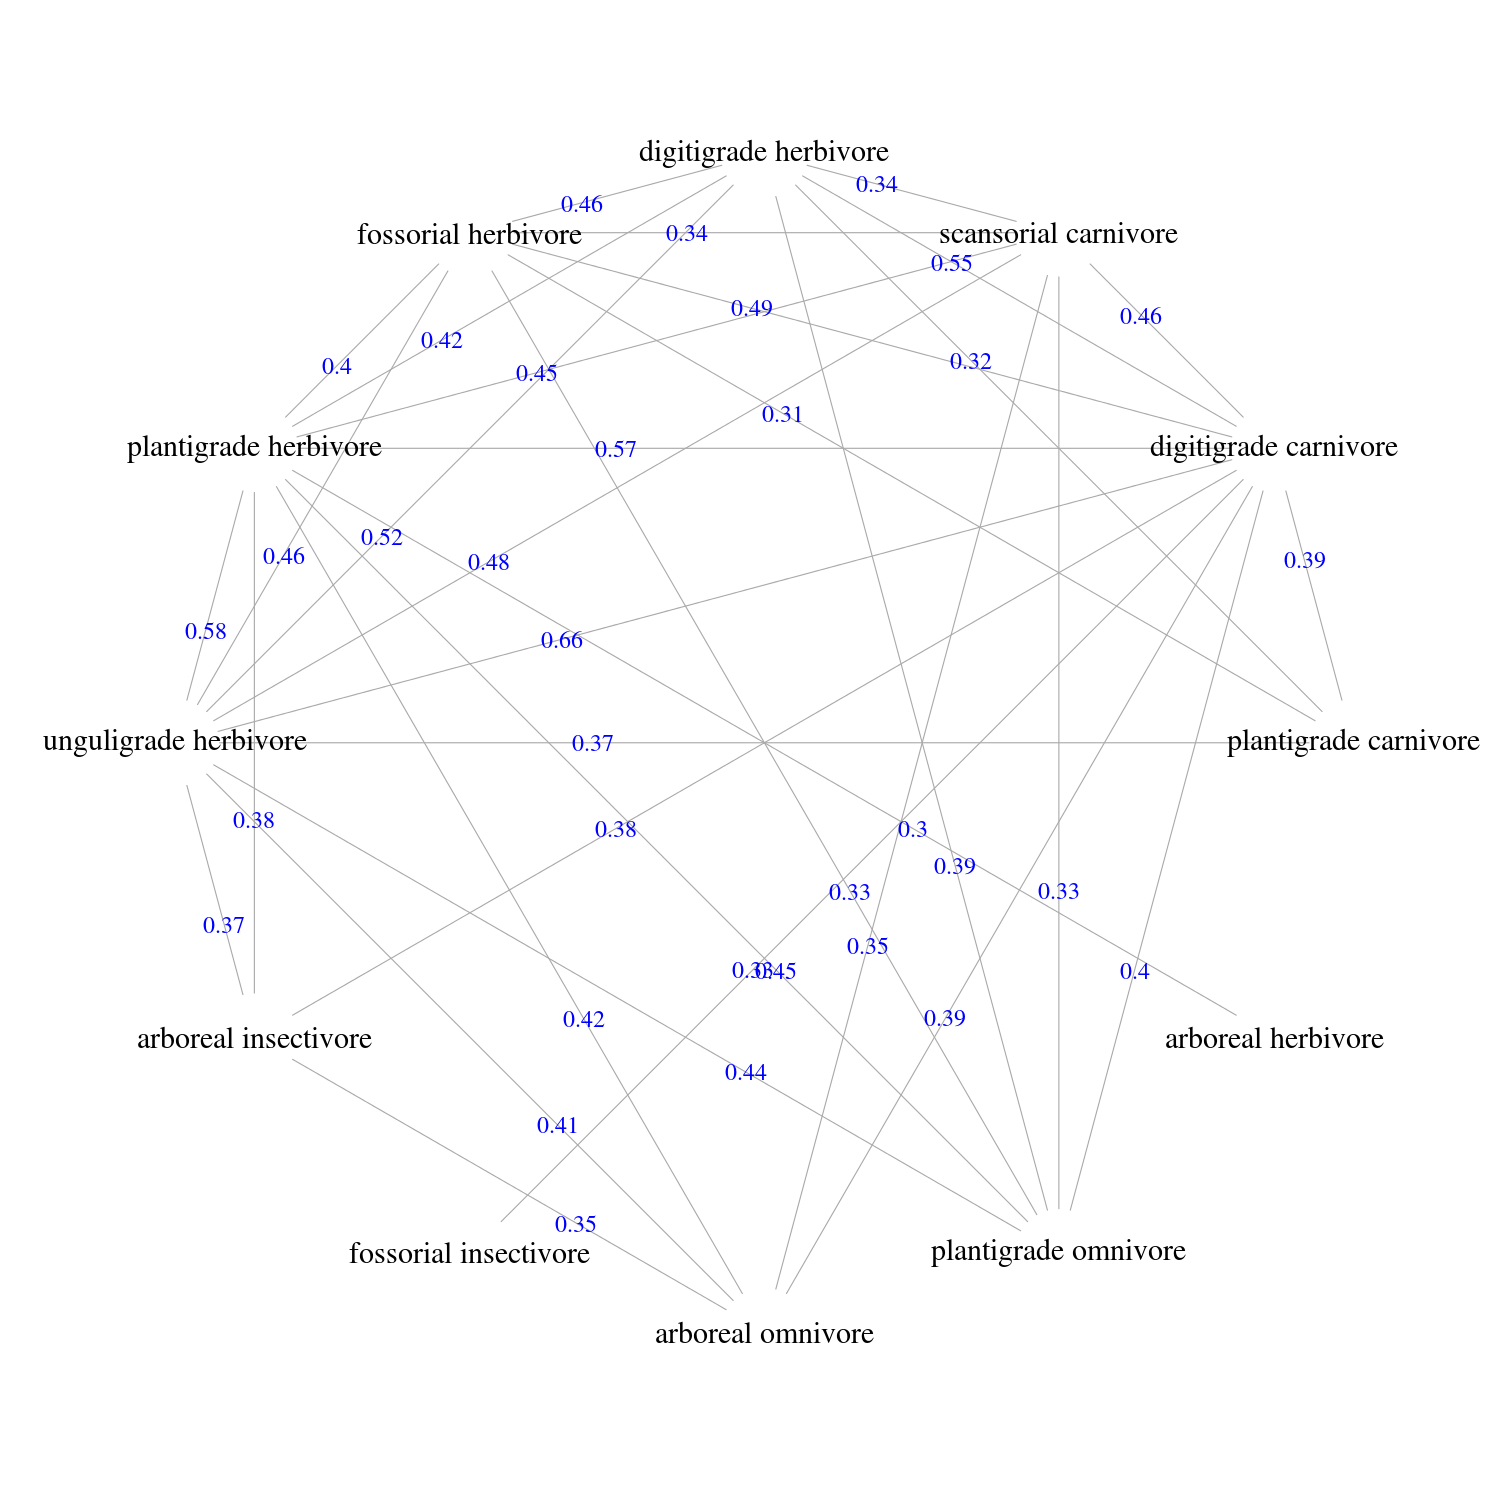
\includegraphics[width=\textwidth,height=\textheight,keepaspectratio=true]{figure/origin_sig_corr}
  \caption{Graph depicting the correlations between functional group origination probabilities that are found with at least weak support (P\(>\)0.8). Nodes indicate the functional group, while edges indicate the cross-correlations. Edges are labeled with the median of the posterior estimates for that correlation.} 
  \label{fig:origin_sig_corr}
\end{figure}





% survival
%   individual-level
%     FG time series
The survival probability time-series vary greatly by functional groups with each exhibiting a unique pattern (Fig. \ref{fig:eco_survival}). Interestingly, unlike origination probability (Fig. \ref{fig:eco_origin}), survival probability is frequently estimated with considerable uncertainty. When survival probability is below 0.50 then a species that is present is unlikely to survive from one time unit to the next, while when survival probability is greater than 0.50 species can be expected to survive to the next time unit. Finally, when survival probability is approximately 0.50 then survival and extinction are equally likely. For most mammal functional groups, survival probability is rarely estimated to be greater than 0.50 with any certainty. This result is consistent with the average occurrence being \(<\)1.35 time units per species which means that a plurality of species have only a single temporal occurrence (Fig. \ref{fig:ppc}).

The survival probability for many functional groups is frequently estimated to be between 0.50 and 0.25 (Fig. \ref{fig:eco_survival}). For example, median survival probability scansorial carnivores is approximately 0.25-0.30 for the entire time series which indicates that there is no best or worst time for this functional groups survival. Similar patterns can be observed for mean survival probability of fossorial insectivores, plantigrade insectivores, and scansorial herbivores.

There are six functional groups that demonstrate an overall decline in survival probability: arboreal carnivores, arboreal herbivores, arboreal insectivores, fossorial herbivores, plantigrade carnivores, and plantigrade omnivores. This result does not mean that these functional groups have identical survival probability time series or all decline at the same time, but that these functional gropus have approximately monotonic decreases in median survival probability for the Cenozoic.

A common feature of multiple functional group's survival probability time-series is a peak in survival during the Neogene (Fig. \ref{fig:eco_survival}). In most cases, these peaks are estimated with little uncertainty which indicates how apparent this event is. Digitigrade carnivores, digitigrade herbivores, plantigrade herbivores, scansorial insectivores, unguligrade herbivores, and unguligrade omnivores all peak in survival probability by the Monroecreekian 26.3 Mya. This peak in survival means that species of these functional groups which are unlikely to go extinct at this point, potentially indicating favorable environmental conditions for these groups at the Paleogene-Neogene transition. Additionally, this peak does not coincide with the change from one plant phase to another (Table \ref{tab:plant_def}). 
\begin{figure}[ht]
  \centering
  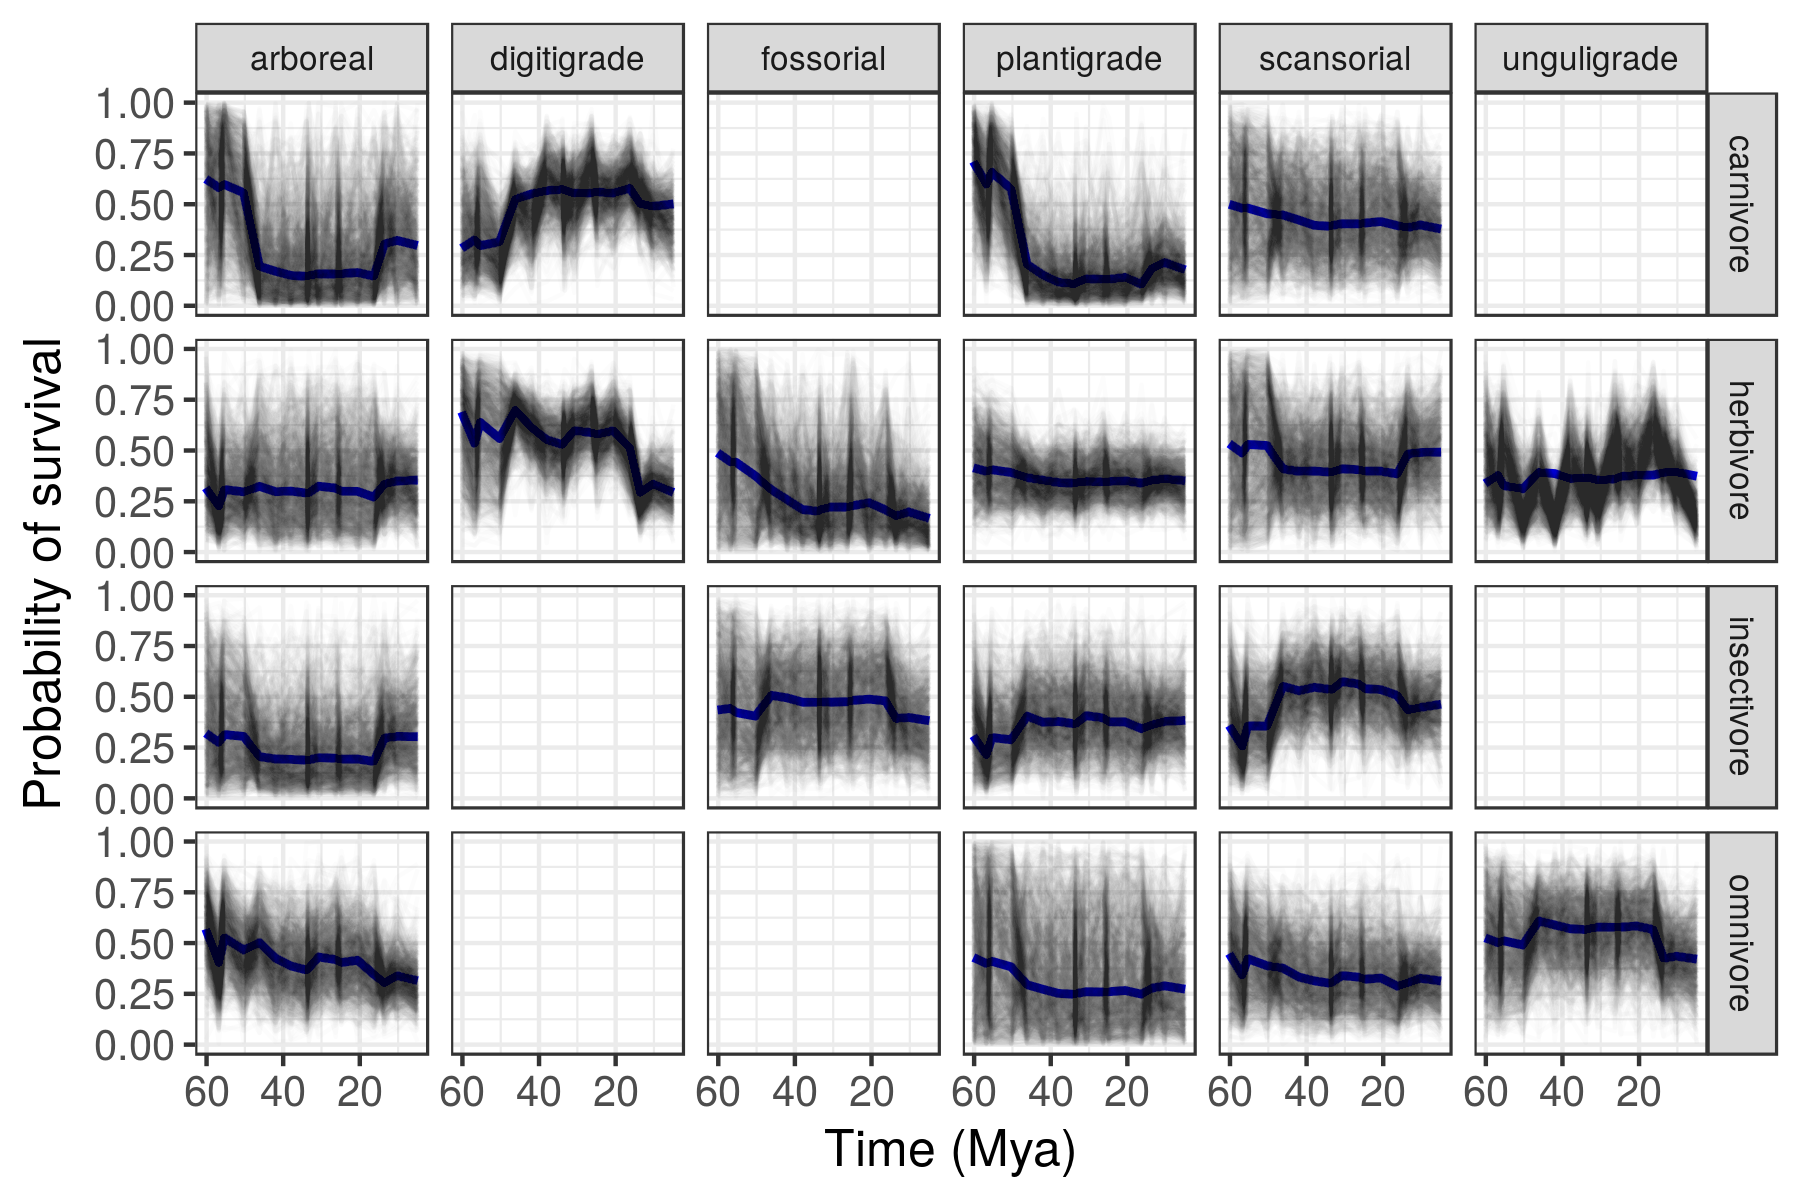
\includegraphics[width=\textwidth,height=0.4\textheight,keepaspectratio=true]{figure/ecotype_survival_bd}
  \caption{Probability of a species continued survival based on functional groups. Survival probability is graphed as 100 time-series drawn from the model's posterior estimates. A greater density of the posterior estimates indicates increased certainty. The blue line is the mean survival probability as predicted by just the group-level predictors. The columns are by locomotor category and rows by dietary category.}
  \label{fig:eco_survival}
\end{figure}

%     order effect
There is virtually no effect of species' order on log-odds of survival (Fig. \ref{fig:order_surv}). All of orders have approximately equal posterior distributions for their estimated effects on log-odds of observation, all of which are centered strongly on 0. These results not only indicate that survival is much more dependent on when a is present species but also its functional ecology as opposed to its taxonomic similarity. 
\begin{figure}[ht]
  \centering
  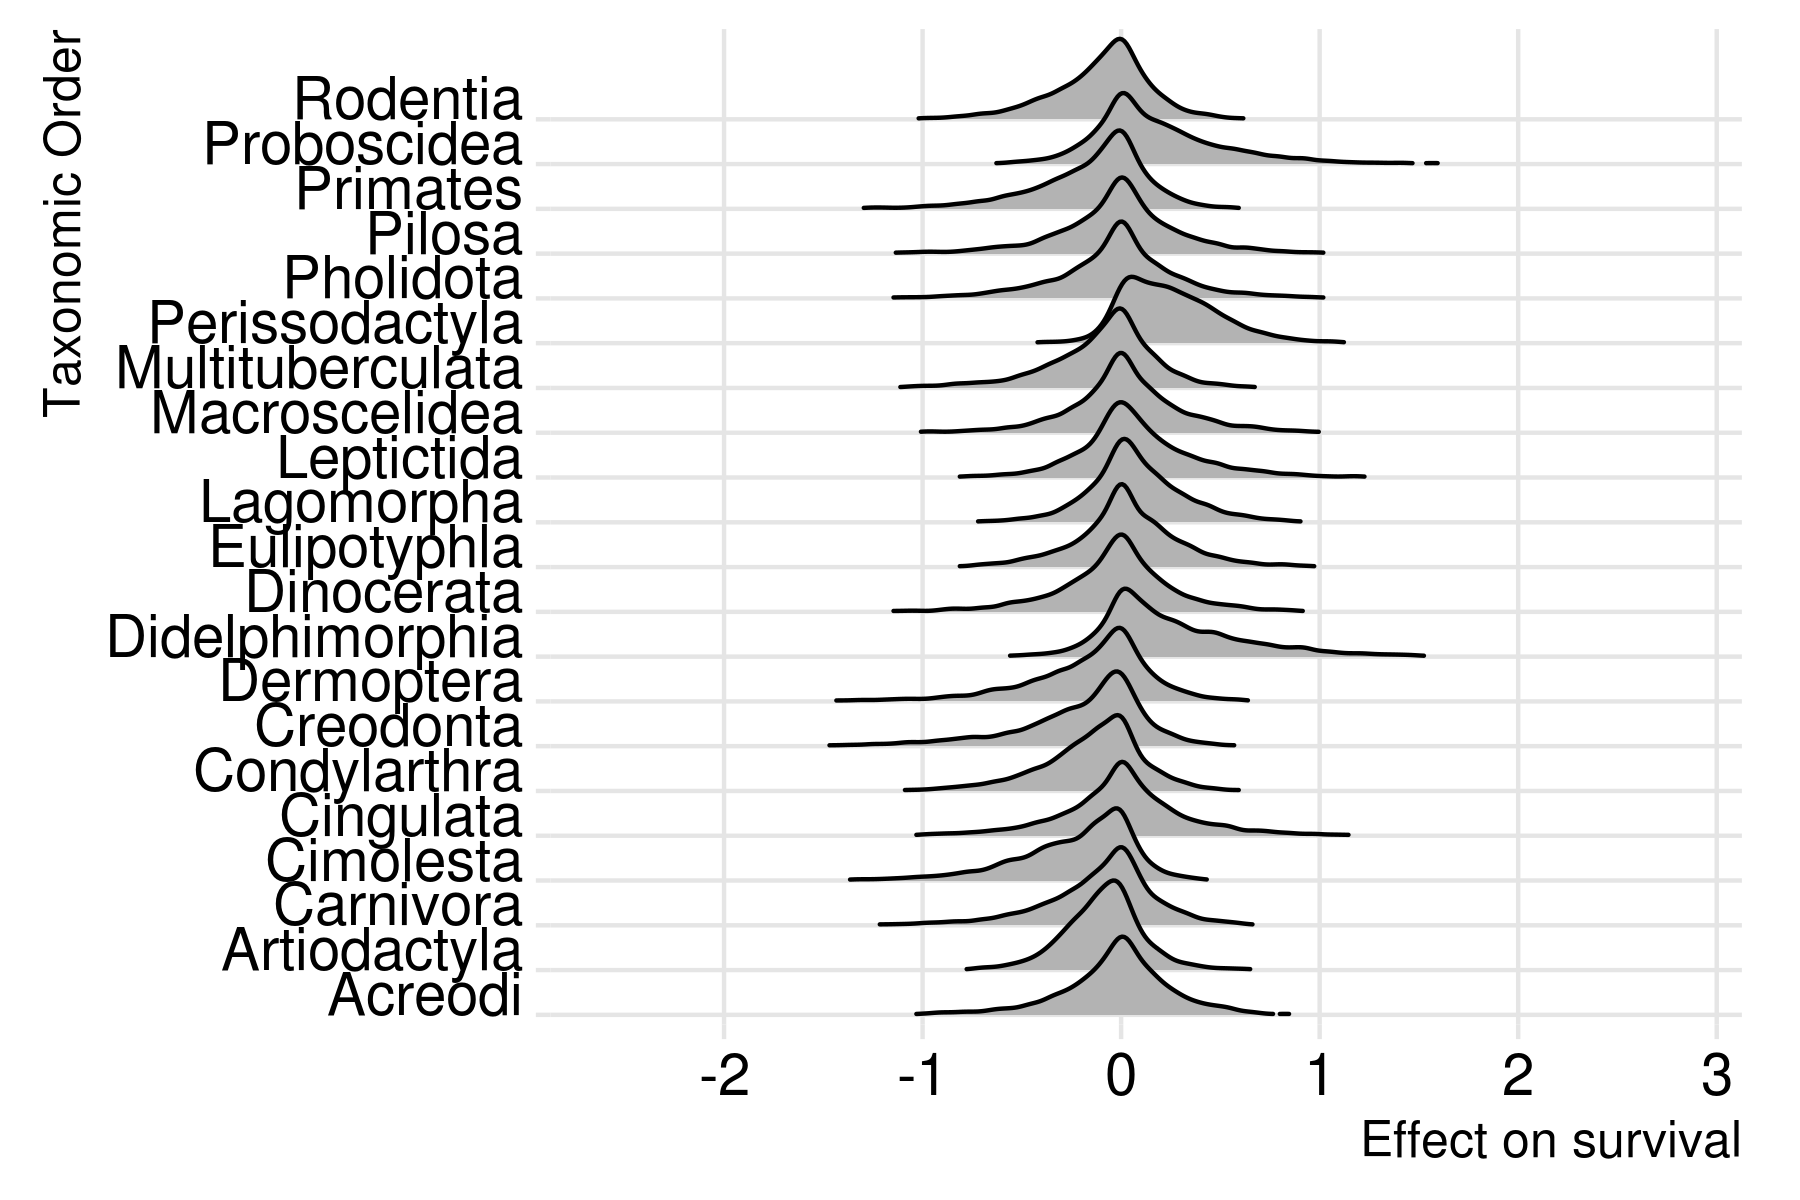
\includegraphics[width=\textwidth,height=0.4\textheight,keepaspectratio=true]{figure/order_survival_bd}
  \caption{Differences in log-odds of survival based on mammal orders. Positive values correspond to greater log-odds survival than average, while negative values correspond to lower log-odds of survival than average.}
  \label{fig:order_surv}
\end{figure}

%     mass effect
\uppercase{mass effect}
%Species mass is estimated to possibly have a positive relationship with survival probability (P(\(\beta^{\pi} > 0\)) = 0.88; Fig. \ref{fig:mass_survival}). This result means that it is plausible that species with greater than average mass have a greater extinction risk than those of average or below average mass. This relationship is the opposite of that predicted by CITATION and is in contrast to those from CITATION. However, because of the marginal plausibility of this result, it is not a strong refutation of these previous results. Instead, it points to why there has been confusion as to the effect of mass on survival; this effect might be very small relative to other factors such as functional ecology and thus difficult to estimate the nature of this relationship with high certainty.
\begin{figure}[ht]
  \centering
  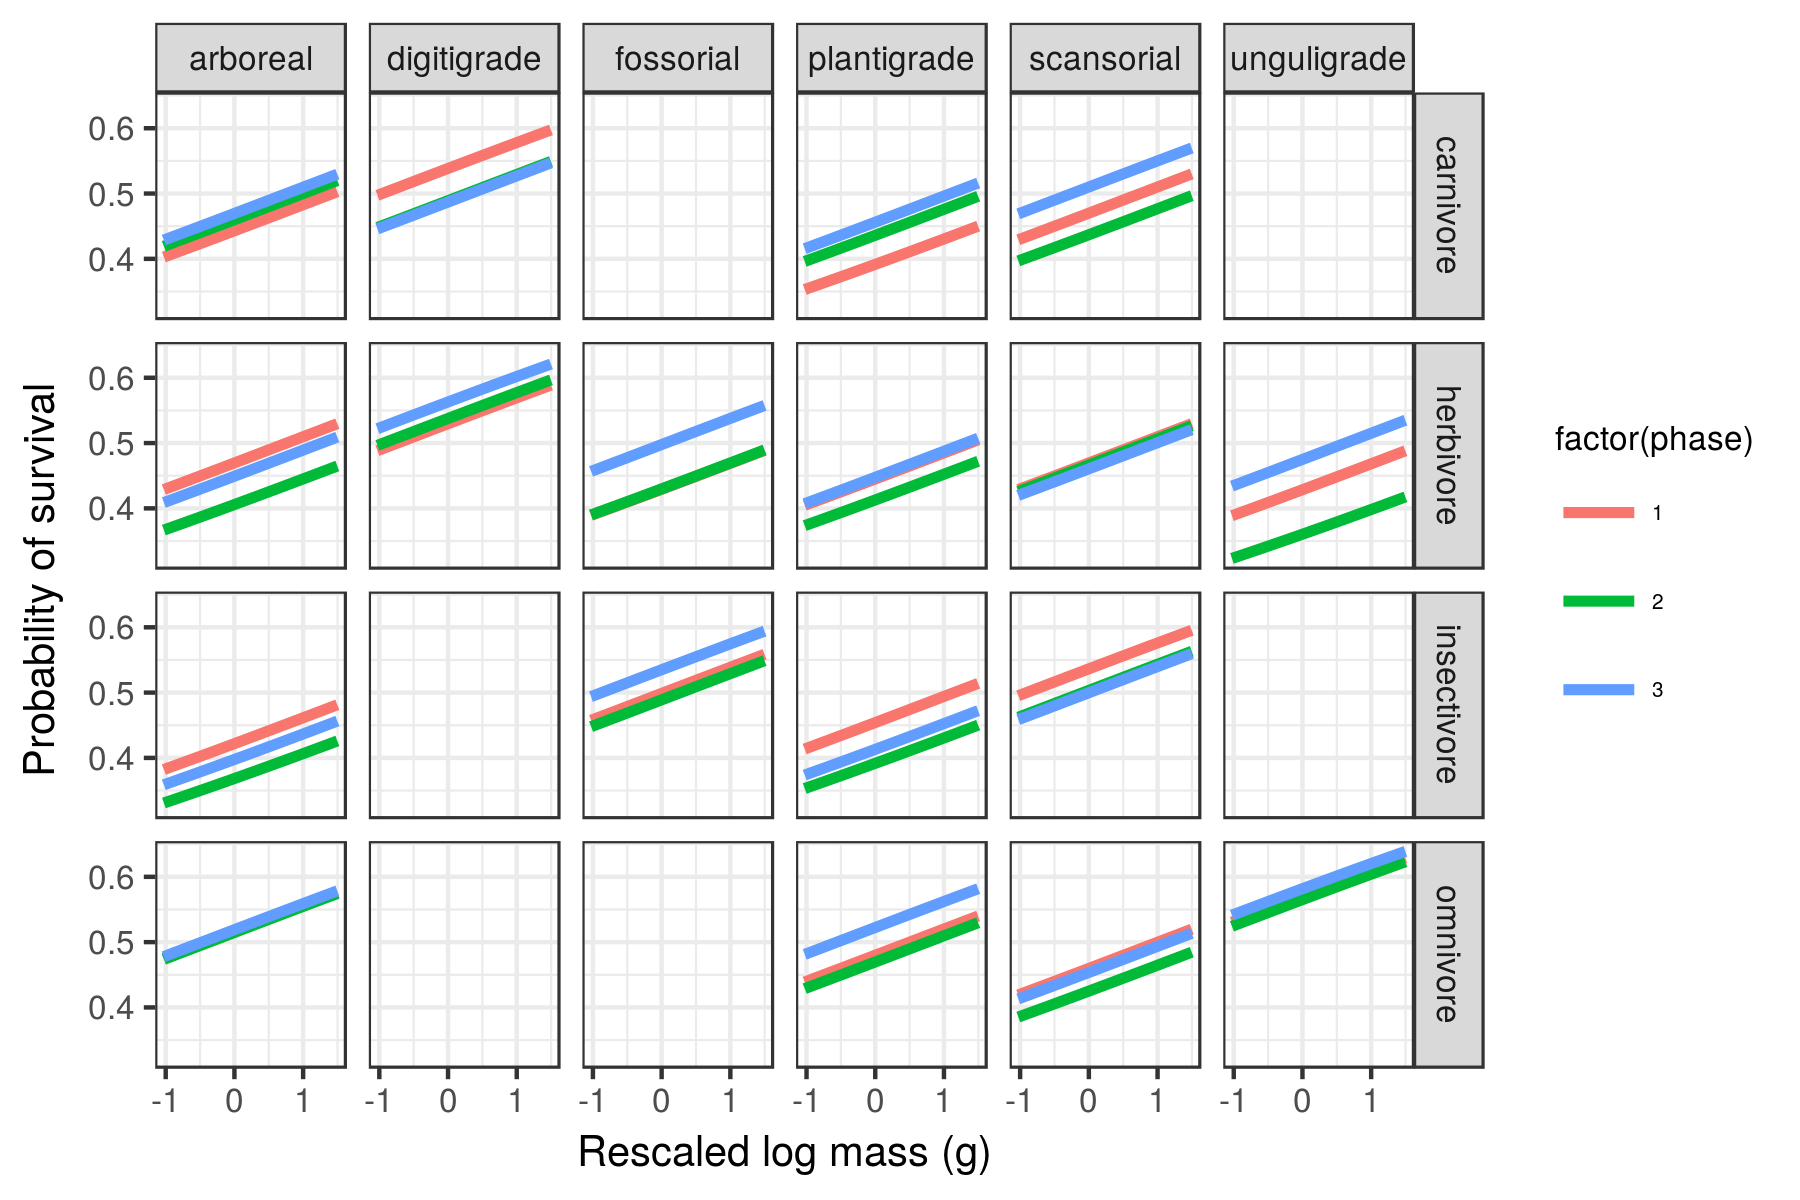
\includegraphics[width=\textwidth,height=0.4\textheight,keepaspectratio=true]{figure/mass_on_surv_bd}
  \caption{Mean estimates of the effect of species' mass on the probability of a species surviving, plotted for each of the three plant phases. While the effect of mass is considered constant over time, each plant phases corresponds to a different intercept of the relationship between mass and survival. The three plant phases are indicated by the color of the line. Mass has been log-transformed, centered, and rescaled; this means that a mass of 0 corresponds to the mean of log-mass of all observed species and that mass is in standard deviation units. For clarity, only the mean of these estimates.}
  \label{fig:mass_survival}
\end{figure}

%   group-level
%     temperature and plant phase
There is no evidence, weak or storng, that the group-level covariates have an effect on functional group survival probabilities (Fig. \ref{fig:group_surv_bd}). This is the case for the plant phases (Table \ref{tab:surv_plant}) and global temperature (Table \ref{tab:surv_temp}). These results are congruent no association between extinction and global temperature CITATION ALROY or as well as results indicating there is no consistent, unidirectional relationship between extinction and global temperature CITATION. 
\begin{figure}[ht]
  \centering
  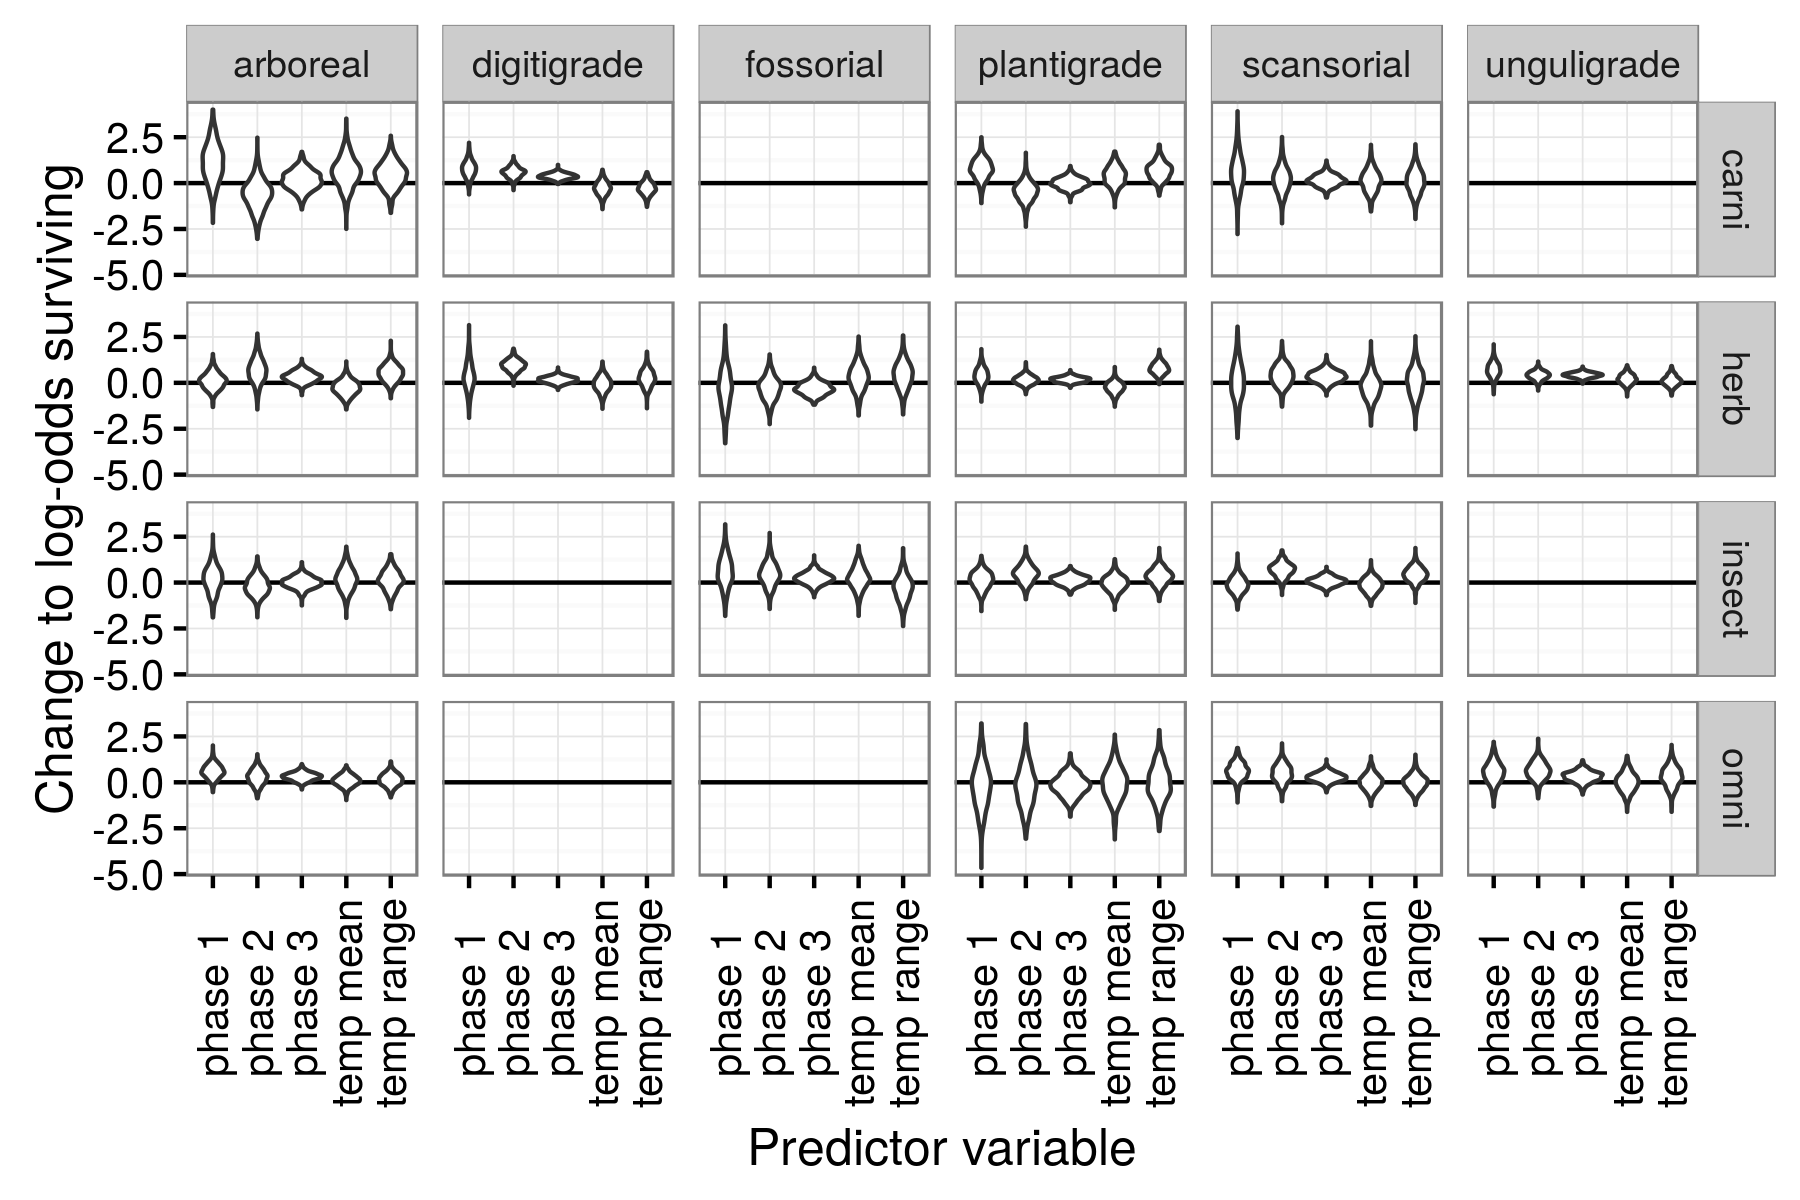
\includegraphics[width=\textwidth,height=0.4\textheight,keepaspectratio=true]{figure/group_on_survival_bd}
  \caption{Estimated effects of the group-level covariates describing environmental context on log-odds of species survival. The violin densities that are plotted are based on 1000 samples from the approximate posterior. The color of the violin corresponds to the probability that the covariates effect is estimated to be greater than 0; red values correspond to greater than 0.50 probability of being positive, blue values correspond to less than 0.50 probability of being positive.} 
  \label{fig:group_surv_bd}
\end{figure}

% make these tables appendix
\begin{table}[ht]
  \centering
  \caption[Posterior probablity estimates of differences in survival by plant phase]{Probability of one plant phase having greater log-odds of survival than another. The first two columns are comparisons of that posterior estimate to zero, which corresponds to the probability of that plant phase having a greater log-odds of survival when compared to the Miocene-Pleistocene. The final columnn corresponds to the comparison in log-odds of survival between the Eocene-Miocene and the Paleocene-Eocene.} 
  \label{tab:surv_plant}
  \begin{tabular}{ l r r r }
    \hline
    & P(Eo.Mi $>$ 0) & P(Pa.Eo $>$ 0) & P(Eo.Mi $>$ Pa.Eo) \\ 
    \hline
    arboreal carnivore & 0.350 & 0.617 & 0.317 \\ 
    digitigrade carnivore & 0.617 & 0.366 & 0.676 \\ 
    plantigrade carnivore & 0.429 & 0.698 & 0.305 \\ 
    scansorial carnivore & 0.471 & 0.455 & 0.504 \\ 
    arboreal herbivore & 0.529 & 0.401 & 0.606 \\ 
    digitigrade herbivore & 0.634 & 0.486 & 0.600 \\ 
    fossorial herbivore & 0.548 & 0.506 & 0.534 \\ 
    plantigrade herbivore & 0.403 & 0.423 & 0.478 \\ 
    scansorial herbivore & 0.383 & 0.494 & 0.417 \\ 
    unguligrade herbivore & 0.529 & 0.503 & 0.517 \\ 
    arboreal insectivore & 0.421 & 0.416 & 0.507 \\ 
    fossorial insectivore & 0.547 & 0.465 & 0.555 \\ 
    plantigrade insectivore & 0.517 & 0.409 & 0.569 \\ 
    scansorial insectivore & 0.600 & 0.377 & 0.658 \\ 
    arboreal omnivore & 0.620 & 0.486 & 0.597 \\ 
    plantigrade omnivore & 0.451 & 0.492 & 0.465 \\ 
    scansorial omnivore & 0.532 & 0.464 & 0.551 \\ 
    unguligrade omnivore & 0.639 & 0.538 & 0.577 \\ 
    \hline
  \end{tabular}
\end{table}

\begin{table}[ht]
  \centering
  \caption[Posterior probablity of effects of temperature on survival]{Probability that the two temperature covariates have an effect on the log-odds of functional group survival. Values greater than 0.50 correspond to the probability of that effect having positive relationship with survival, while values less than 0.5 correspond increasing certainty that that covariate has a negative relationship with survival.}
  \label{tab:surv_temp}
  \begin{tabular}{ l r r }
    \hline
    & \(P(\gamma_{temp\ mean} > 0)\) \\
    \hline
    arboreal carnivore & 0.577 \\ 
    digitigrade carnivore & 0.444 \\ 
    plantigrade carnivore & 0.642 \\ 
    scansorial carnivore & 0.491 \\ 
    arboreal herbivore & 0.433 \\ 
    digitigrade herbivore & 0.507 \\ 
    fossorial herbivore & 0.545 \\ 
    plantigrade herbivore & 0.438 \\ 
    scansorial herbivore & 0.452 \\ 
    unguligrade herbivore & 0.528 \\ 
    arboreal insectivore & 0.441 \\ 
    fossorial insectivore & 0.515 \\ 
    plantigrade insectivore & 0.425 \\ 
    scansorial insectivore & 0.363 \\ 
    arboreal omnivore & 0.493 \\ 
    plantigrade omnivore & 0.515 \\ 
    scansorial omnivore & 0.454 \\ 
    unguligrade omnivore & 0.531 \\ 
    \hline
  \end{tabular}
\end{table}

%     correlation
None of the time-series of functional group survival probability are estimated to be either positively or negatively correlated (Fig. \ref{fig:survival_corr}). This result indicates that functional groups probably have ultimately independent survival histories for the entire study period. As with origination probability, this result does not preclude the possibility of short term similarities in expansion and decline of origination probability or shared peaks and troughs of survival probability. Additionally, if the relationship between two functional groups changes over time (e.g. from positive correlation to negative correlation), then it would yield no overall correlation for the Cenozoic. Finally, it is important to remember that this estimate correlation is based on survival probability and not extinction rate or diversity.
\begin{figure}[ht]
  \centering
  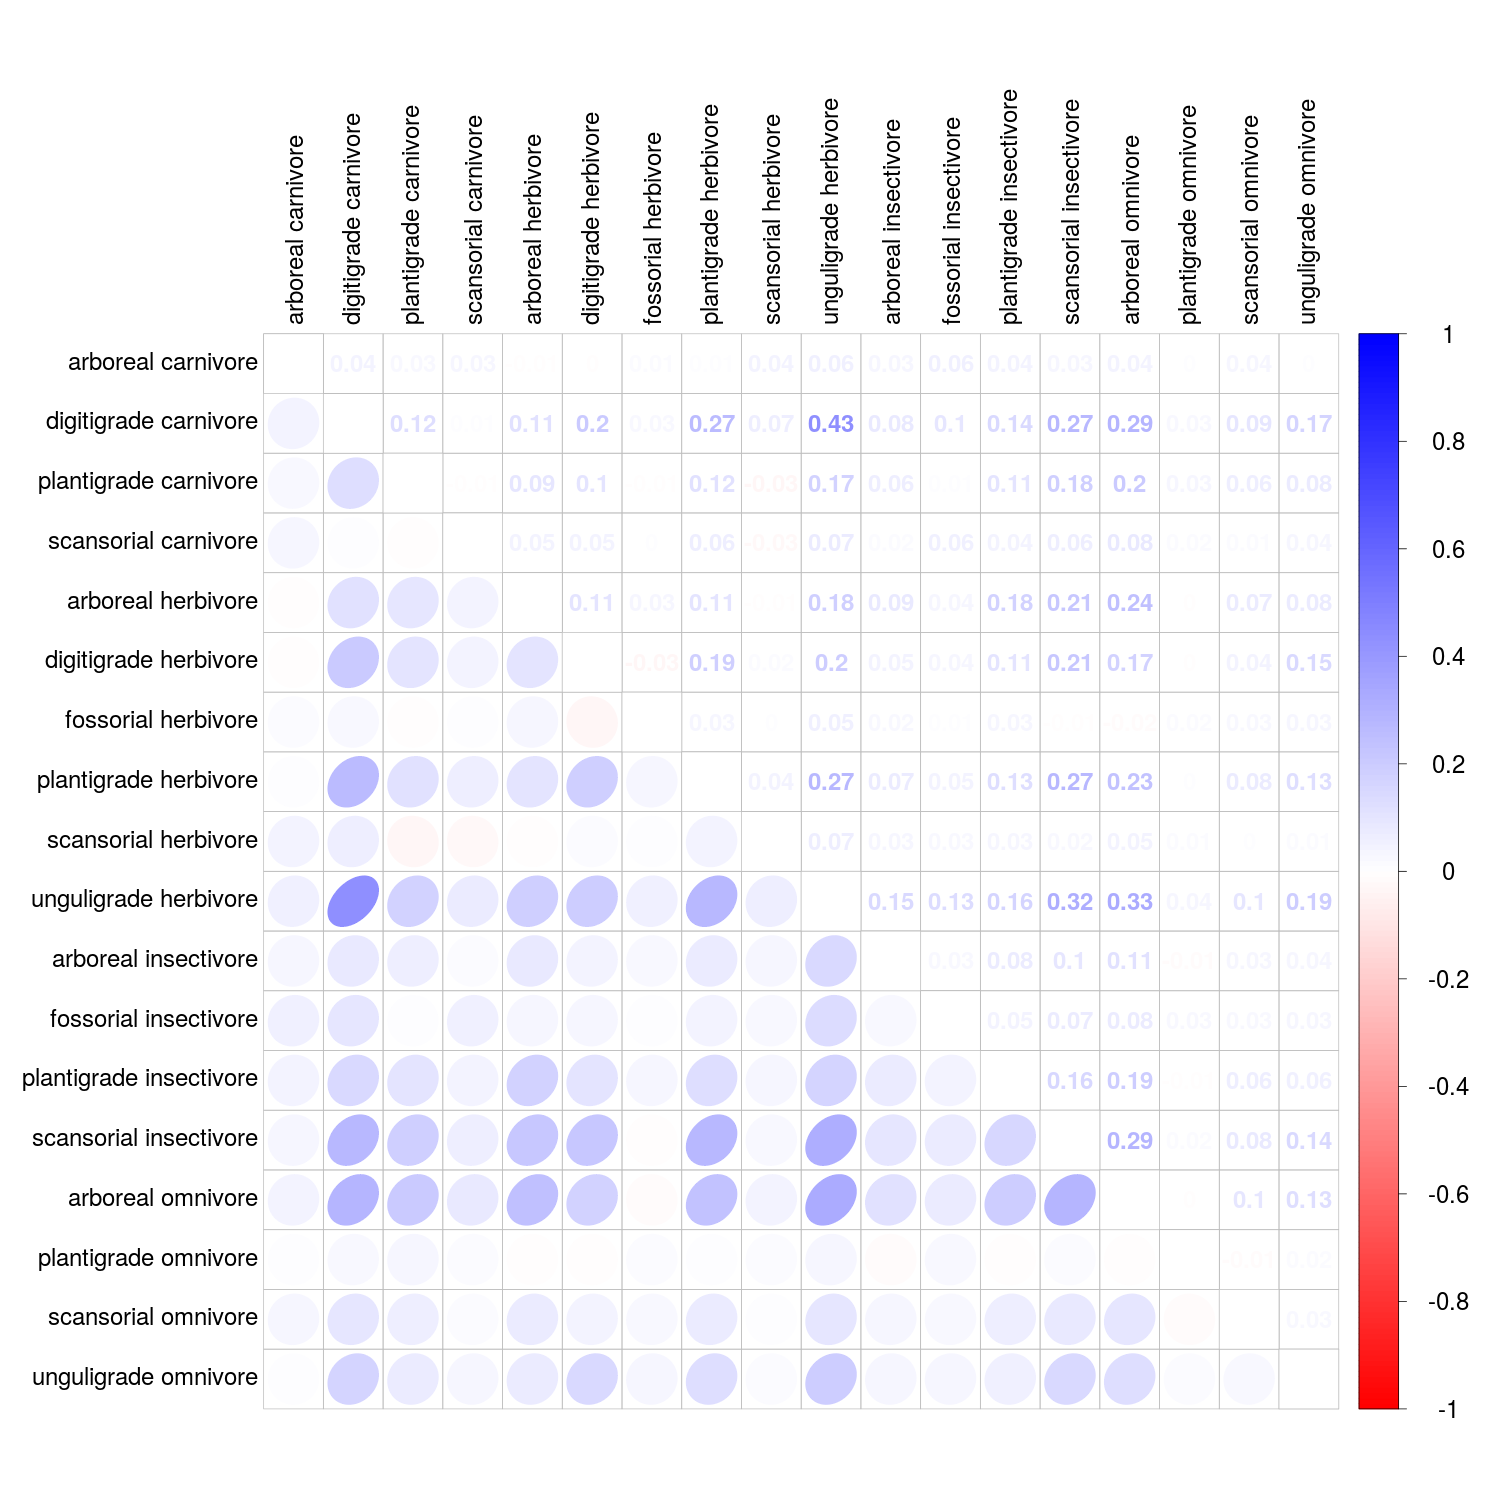
\includegraphics[width=\textwidth,height=\textheight,keepaspectratio=true]{figure/survival_correlation}
  \caption{Posterior estimate of mean correlations in survival probability between the mammal functional groups. The lower triangle of the matrix is populated with ellipses corresponding to the level of correlation between the two functional groups, while the upper triangle of the matrix corresponds to the mean estimate of the correlation between functional groups. Darker values correspond to a greater magnitude of correlation with blue values corresponding to a positive correlation and red values a negative correlation.}
  \label{fig:survival_corr}
\end{figure}






%% HERE
\subsection*{Analysis of diversity}
Standing diversity of the North American mammal species pool estimated from this model exhibits an initial increase in diversity followed by a decrease till approximately the Orellan through the Geringian about 33.9-30.8Mya, after which there is a marked increase till approximately the Barstovian 15Mya after which it decreases slightly till it is equal to the overall mean diversity of the Cenozoic (Fig. \ref{fig:diversity_est}). Per-unit standing diversity is found to be different from average standing diversity for 16 of 18 time-units at P\(>\)0.80, and 14 of 18 at P\(>0.90)\); Table \ref{tab:div_peak}). Diversity is greater than average during the Tiffanian, Wasatchian, Uintan, Hemingfordian, Barsotvian, Clarendonian, and Blancan while diversity is lower than average during the Torrejonian, Clarkforkian, Duchesnean, Chadronian, Orellan, Whitneyan, Geringian, Monroecreekian, and Harrisonian. The nadir of diversity is the between the Orellan and Geringian, while the apex is the Barstovian (Fig. \ref{fig:diversity_est}). Interstingly, the rise in diversity among the sampled species from the Geringian to the Barstovian is unidirectional and is not estimated to have any temporary dips in diversification for that entire approximately 15 million year period.
\begin{figure}[ht]
  \centering
  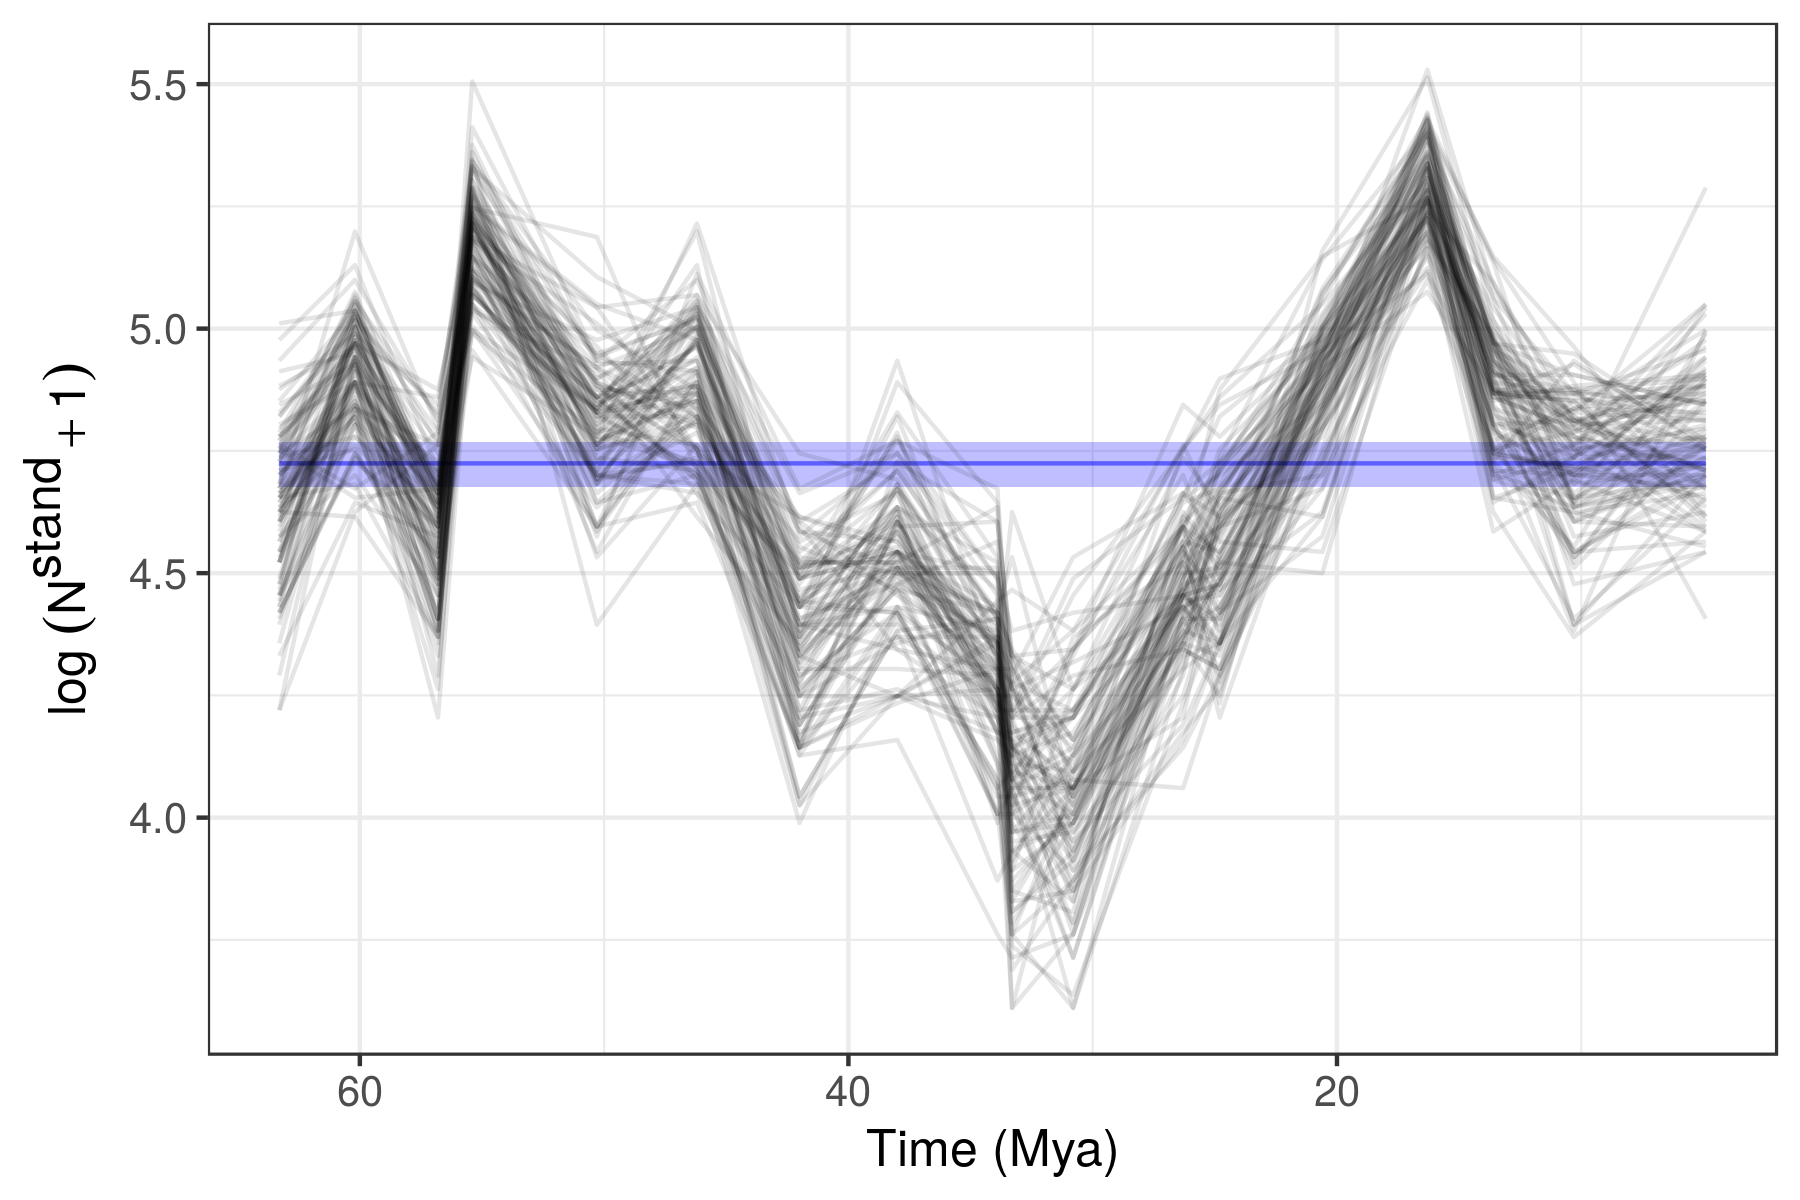
\includegraphics[width=\textwidth,height=0.5\textheight,keepaspectratio=true]{figure/log_diversity}
  \caption{Log diversity}
  \caption{Estimated standing diversity of Cenozoic mammals based on the 1400 species analyzed in this study. Estimates are based on 100 posterior draws of the ``true'' occurrence matrix \(z\) (Table \ref{tab:basic}). The blue horizontal strip corresponds to the median and 80\% credible interval of estimated mean standing diversity for the entire time period studied.} 
  \label{fig:diversity_est}
\end{figure}

\begin{table}[ht]
  \centering
  \caption{Probability that diversity during one NALMA \(N^{stand}_{t}\) is greater than average standing diversity for the whole Cenozoic \(\overline{N^{stand}}\). NALMA is a North American Land Mammal age and is the temporal unit for this study. Values greater than 0.50 indicate support for the diversity at that NALMA being greater than average, while values less than 0.50 indicate support for diversity being less than average. These are listed from oldest to youngest NALMA.}
  \label{tab:div_peak}
  \begin{tabular}{ r r }
    \hline
    NALMA & \(P(N^{stand}_{t} > \overline{N^{stand}})\) \\
    \hline
    Torrejonian & 0.01 \\ 
    Tiffanian & 0.96 \\ 
    Clarkforkian & 0.02 \\ 
    Wasatchian & 1.00 \\ 
    Bridgerian & 0.57 \\ 
    Uintan & 0.89 \\ 
    Duchesnean & 0.00 \\ 
    Chadronian & 0.09 \\ 
    Orellan & 0.00 \\ 
    Whitneyan & 0.00 \\ 
    Geringian & 0.00 \\ 
    Monroecreekian & 0.04 \\ 
    Harrisonian & 0.17 \\ 
    Hemingfordian & 0.96 \\ 
    Barstovian & 1.00 \\ 
    Clarendonian & 0.92 \\ 
    Hemphillian & 0.76 \\ 
    Blancan & 0.98 \\ 
    \hline
  \end{tabular}
\end{table}


Standing diversity when partitioned by ecotype reveals a lot of the complexity behind the pattern of mammal diversity for the Cenozoic (Fig. \ref{fig:ecotype_diversity}). While each functional group has its own unique diveristy history, there are some broad similarities as is similar to the estimates origination and survival probability (Fig. \ref{fig:eco_origin}, \ref{fig:eco_survival}).

Arboreal ecotypes obtain peak diversity early in the Cenozoic and then decline for the rest of the time series, becoming increasingly rare or absent as diversity approaches the Recent (Fig. \ref{fig:ecotype_diversity}). Arboreal herbivores and omnivores obtain peak diversity at the beginning of the Cenozoic then go into decline while remaining a small part of the species pool, while arboreal carnivores and insectivores obtain peak diversity by the WAsatchian 55.4 Mya and then quickly decline and become extremely rare or entirely absent from the species pool. The only arboreal functional group estimated to not experience a complete disappearance from the species pool are arboreal herbivores. This is consistent with increasing extinction risk in the Neogene compared to the Paleogene as proposed by \citet{Smits2015b}.




The diversity of plantigrade insectivores, scansorial insectivores, and scansorial omnivores are estimated to decrease through the Cenozoic (Fig. \ref{fig:ecotype_diversity}). Plantigrade herbivores and scansorial omnivores have peak diversity at the early Cenozoic and reach low diversity by the Orelan and Whitneyan approximately approximately 33 Mya, after which diversity never increases again. In contrast, scansorial omnivores have nearly constant, above average diversity for the beginning of the Cenozoic till approximately Orelan and Whitneyan, after which diversity drops and remaining below average diversity for the rest of the Cenozoic.

The fossorial functional groups included in this study are estimated to be rare or absent absent for the first half of the Cenozoic, fossorial herbivores probably having lower diversity than fossorial insectivores (Fig. \ref{fig:ecotype_diversity}). After fossorial herbivores increase in diversity till the Orelan and Whitneyan approximately 33 Mya, this functional group is estimated to quickly reach approximately constant standing diversity for the rest of the Cenozoic. In contrast, fossorial insectivores increase in diversity starting approximately at the Orelan and Whitneyan and reach max diversity at the Barstovian 16.3 Mya, after which this group declines in diversity.

Plantigrade carnivores, scansorial herbivores and unguligrade omnivores are estimated to maintain near constant standing diversity for most of the Cenozoic (Fig. \ref{fig:ecotype_diversity}). Of these three functional groups, plantigrade carnivores have the greatest variance in standing diversity. Plantigrade carnivores have greater than average standing diversity from the beginning of the Cenozoic till the Bridgerian 50.3 Mya and from the Harrisonian 24.8 Mya till the Barstovian 16.3 Mya. This functional group is estimated to be below average standing diversity from the Bridgerian till the Orelan and Whitneyan approximately 30Mya, and then from the Hemphillian 10.3 Mya till the end of the studied time period. Scansorial herbivores exhibit a similar patterns but with a reversed diversity pattern for the first 30My of the studied period. Instead of near constant diversity, scansorial herbivores are estimated to have lower than average diversity from the beginning of the Cenozoic till the Bridgerian approximately 50.3 Mya, after which this group has approximately average standing diversity for the rest of the Cenozoic. The unguligrade omnivore functional group has slightly elevated diversity at the beginning of the Cenozoic and a possible decrease in diversity after the Barstovian approximately 16.3 Mya.

Scansorial carnivores and plantigrade herbivores have below average standing diversity from the beginning of the Cenozoic till the Hemingfordian approximately 20.6 Mya, after which both functional groups increase in diversity till being well above average by the end of the study period (Fig. \ref{fig:ecotype_diversity}). Plantigrade omnivores are estimated to be absent or extremely rare in the species pool, only increasing in standing diversity beginning at the Hemingfordian approximately 24.8 Mya. In contrast, scansorial carnivores are estimated to have been a rare but constant part of the species pool diversity for the entire Cenozoic with an increase at the Hemingfordian.

Digitigrade carnivores, plantigrade herbivores, and unguligrade herbivores functional groups maintain relatively high standing diversity through out the entire Cenozoic though each exhibits periods of greater than average and below average standing diversity (Fig. \ref{fig:ecotype_diversity}). Digitigrade carnivore diversity is estimated to begin the study period below average and then quickly rise to the first peak in diversity at the Wasatchian 55.4 Mya. After this, ditigrade carnivore diversity decreases to below average diversity till the Orellan and Whitneyan approximately 33 Mya, after which diversity increases till a second greater peak in diversity at the Barstovian 16.3 Mya. After this second peak in diversity, ditigrade carnivore diversity declines until the end of the study period. Unguligrade herbivores exhibit a similar pattern though with considerably less uncertainty. In contrast, while plantigrade herbivores have a similar increase and peak in diversity during the first half of the Cenozoic, the functional group does not experience a second peak in functional diversity till the end of the study period. Additionally, plantigrade herbivores have a longer period of above average standing diveristy during the first half of the Cenozoic, only experiencing a decrease in diversity starting at the Orellan and Whitneyan approximately 33Mya.

The digitigrade herbivore functional group is estimated to be the only group with a near constant increase in standing diversity through most of the Cenozoic (Fig. \ref{fig:ecotype_diversity}). There are two periods of decrease in the standing diversity of digitigrade herbivores: from the start of the study period will the Wasatchian 55.4 Mya, and a sudden decrease at the Clarendonian 13.6 Mya. Beyond these two decreases, this functional group exhibits a remarkable increase in diversity from relative rarity at the Wasatchian and Bridgerian till peak diversity at the Hemingfordian and Barstovian. Diversity even appears to begin to rebound after the sudden decrease at the Clarendonian 13.6 Mya.
\begin{figure}[ht]
  \centering
  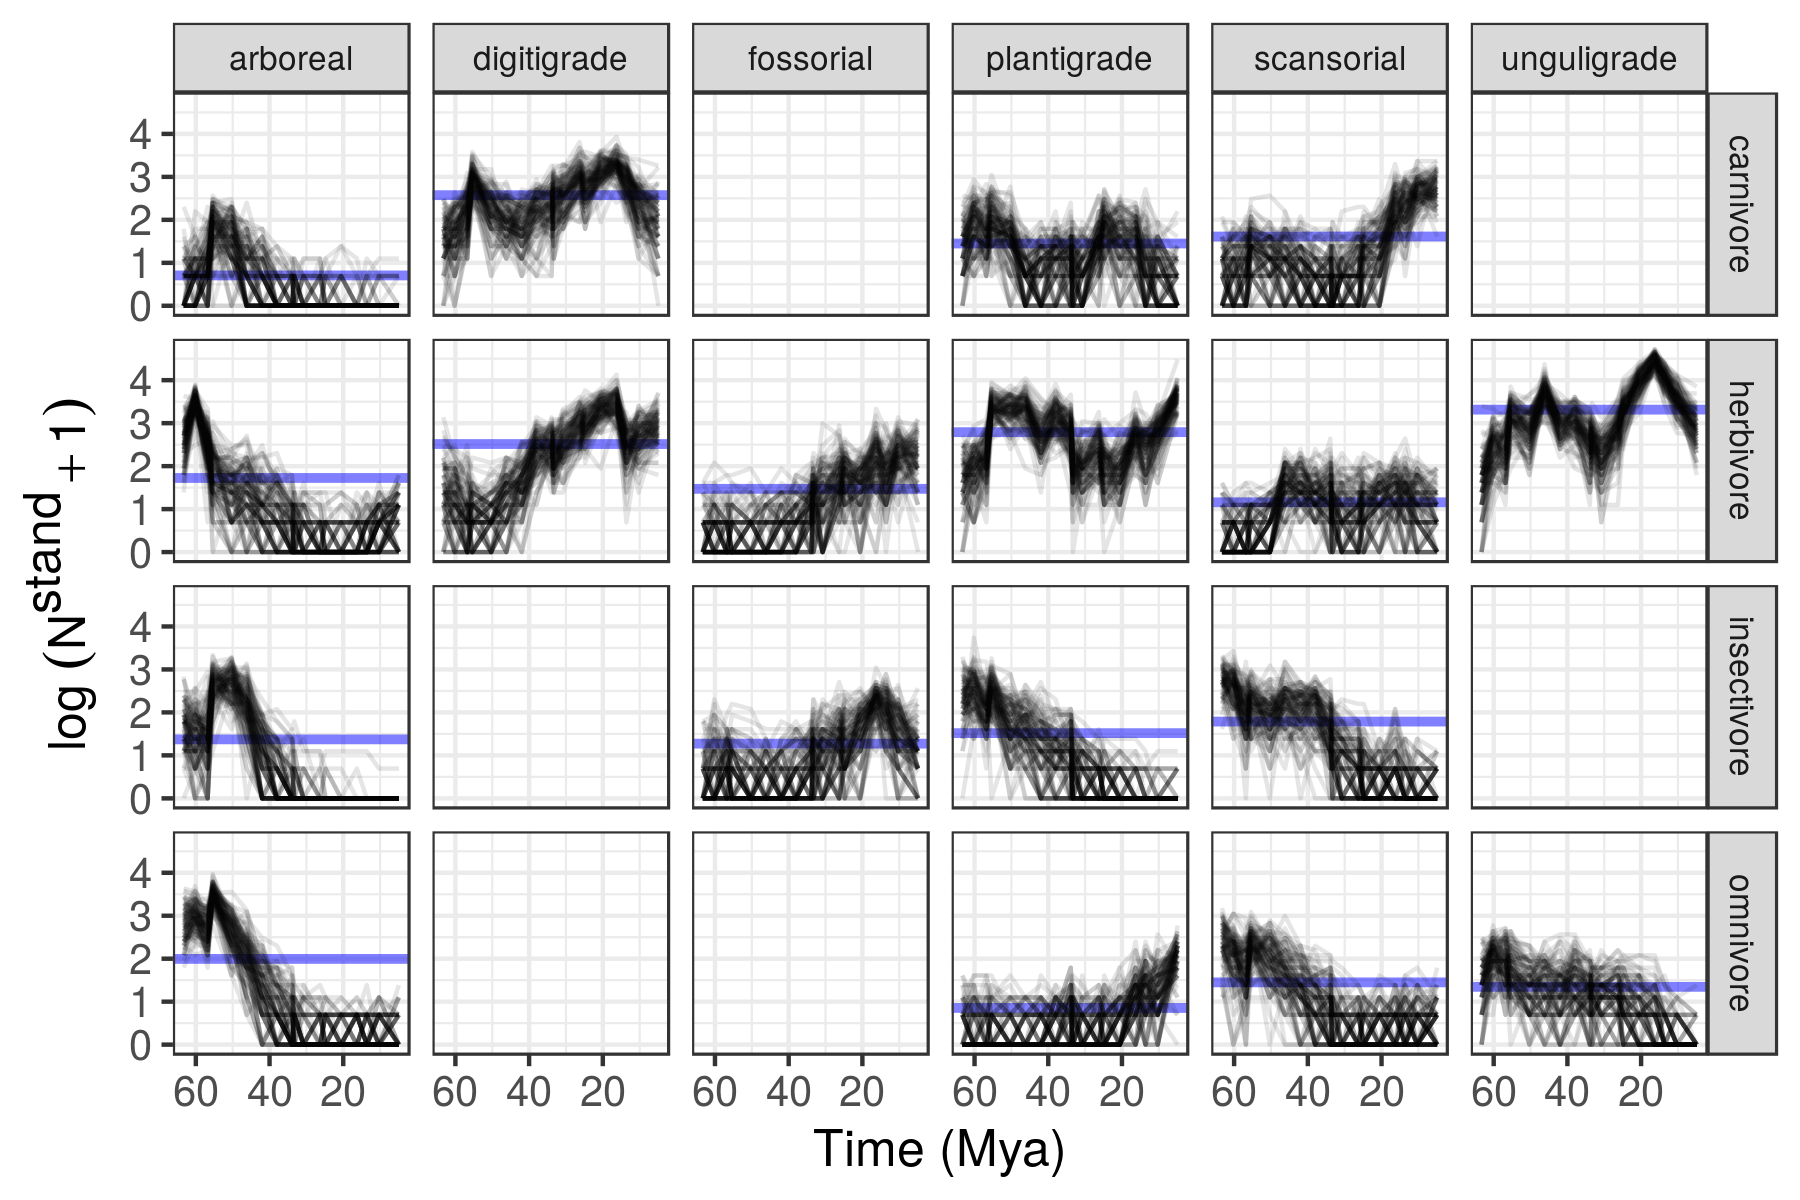
\includegraphics[width=\textwidth,height=0.5\textheight,keepaspectratio=true]{figure/ecotype_diversity}
  \caption{Estimated standing log-diversity of North American mammals by functional group for the Cenozoic. Diversity is represented as 100 posterior draws plotted over time. Density of time-series indicates congruence in estimates. The blue line corresponds to average standing diversity for that functional group for the entire Cenozoic.} 
  \label{fig:ecotype_diversity}
\end{figure}



The waxing and waning of the mammal ecotypes is obvious when comparing changes to estimated relative log-mean diversity (Fig. \ref{fig:ecotype_relative}). While the relative diversity of functional groups changes gradually over time, there are definite patterns associated with a few functional groups and axes of functional diversity that are interesting. There are many expansions and retractions of functional group relative diversity, some of which are coincidental. Only in the case of digitigrade carnivores, plantigrade herbivores, and scansorial omnivores are their functional groups are maintained as relatively constant proportions of the species pool (Fig. \ref{fig:ecotype_relative}).

% increase in the species pool
Eight of the 18 functional groups expand in relative diversity over the Cenozoic (Fig. \ref{fig:ecotype_relative}). Digitigrade herbivores have an obvious increase in relative diversity at the Uintan 46.2 Mya, after which it remains a substantial part of the species pool. Fossorial herbivores, and fossorial insectivores increase in relative diversity at the Orellan and Whitneyan approximately 33 Mya, after which these groups are maintained as parts of the species pool. Plantigrade omnivores, and scansorial carnivores are both a relatively small fraction of the species pool until the Hemingfordian 20.6 Mya where these functional groups increase in relative diversity for the rest of the time analyzed. Scansorial herbivores expand their relative diversity starting at the Harrisonian 24.8 Mya, after which this functional group has an approximately constant relative diversity. Scansorial insectivores experience in increase in relative diversity after the Bridgerian 50.3 Mya. Finally, unlike other functional groups, unguligrade herbivores slowly increase in their relative diversity for the entire Cenozoic.

% decrease in the species pool
Six of the 18 functional groups are estimated to experience a decrease in relative diversity over the Cenozoic (Fig. \ref{fig:ecotype_relative}). As expected from the diversity time-series for the functional groups (Fig. \ref{fig:ecotype_diversity}), the relative diversity of all four arboreal functional groups declines from the beginning of the Cenozoic until the Orellan and Whitneyan approximately 33 Mya, after which only arboreal herbivores remain in any capacity (Fig. \ref{fig:ecotype_relative}). In addition to the arboreal groups, there are other functional groups which decrease in relative diversity over the Cenozoic (Fig. \ref{fig:ecotype_relative}). Plantigrade carnivores are a relatively constant portion of the species pool until after the Barstovian 16.3 Mya, after which this functional group decreases in relative diversity. Plantigrade insectivores decrease in their relative diversity, experience greatest winnowing starting approximately at the Geringian till the Barstovian, after which this functional group becomes absent from the species pool. Finally, unguligrade omnivores begin to decrease in relative diversity starting at the Hemingfordian 20.6 Mya, after which they continue to decrease until they are only a small portion of the relative diversity of the species pool.
\begin{figure}[ht]
  \centering
  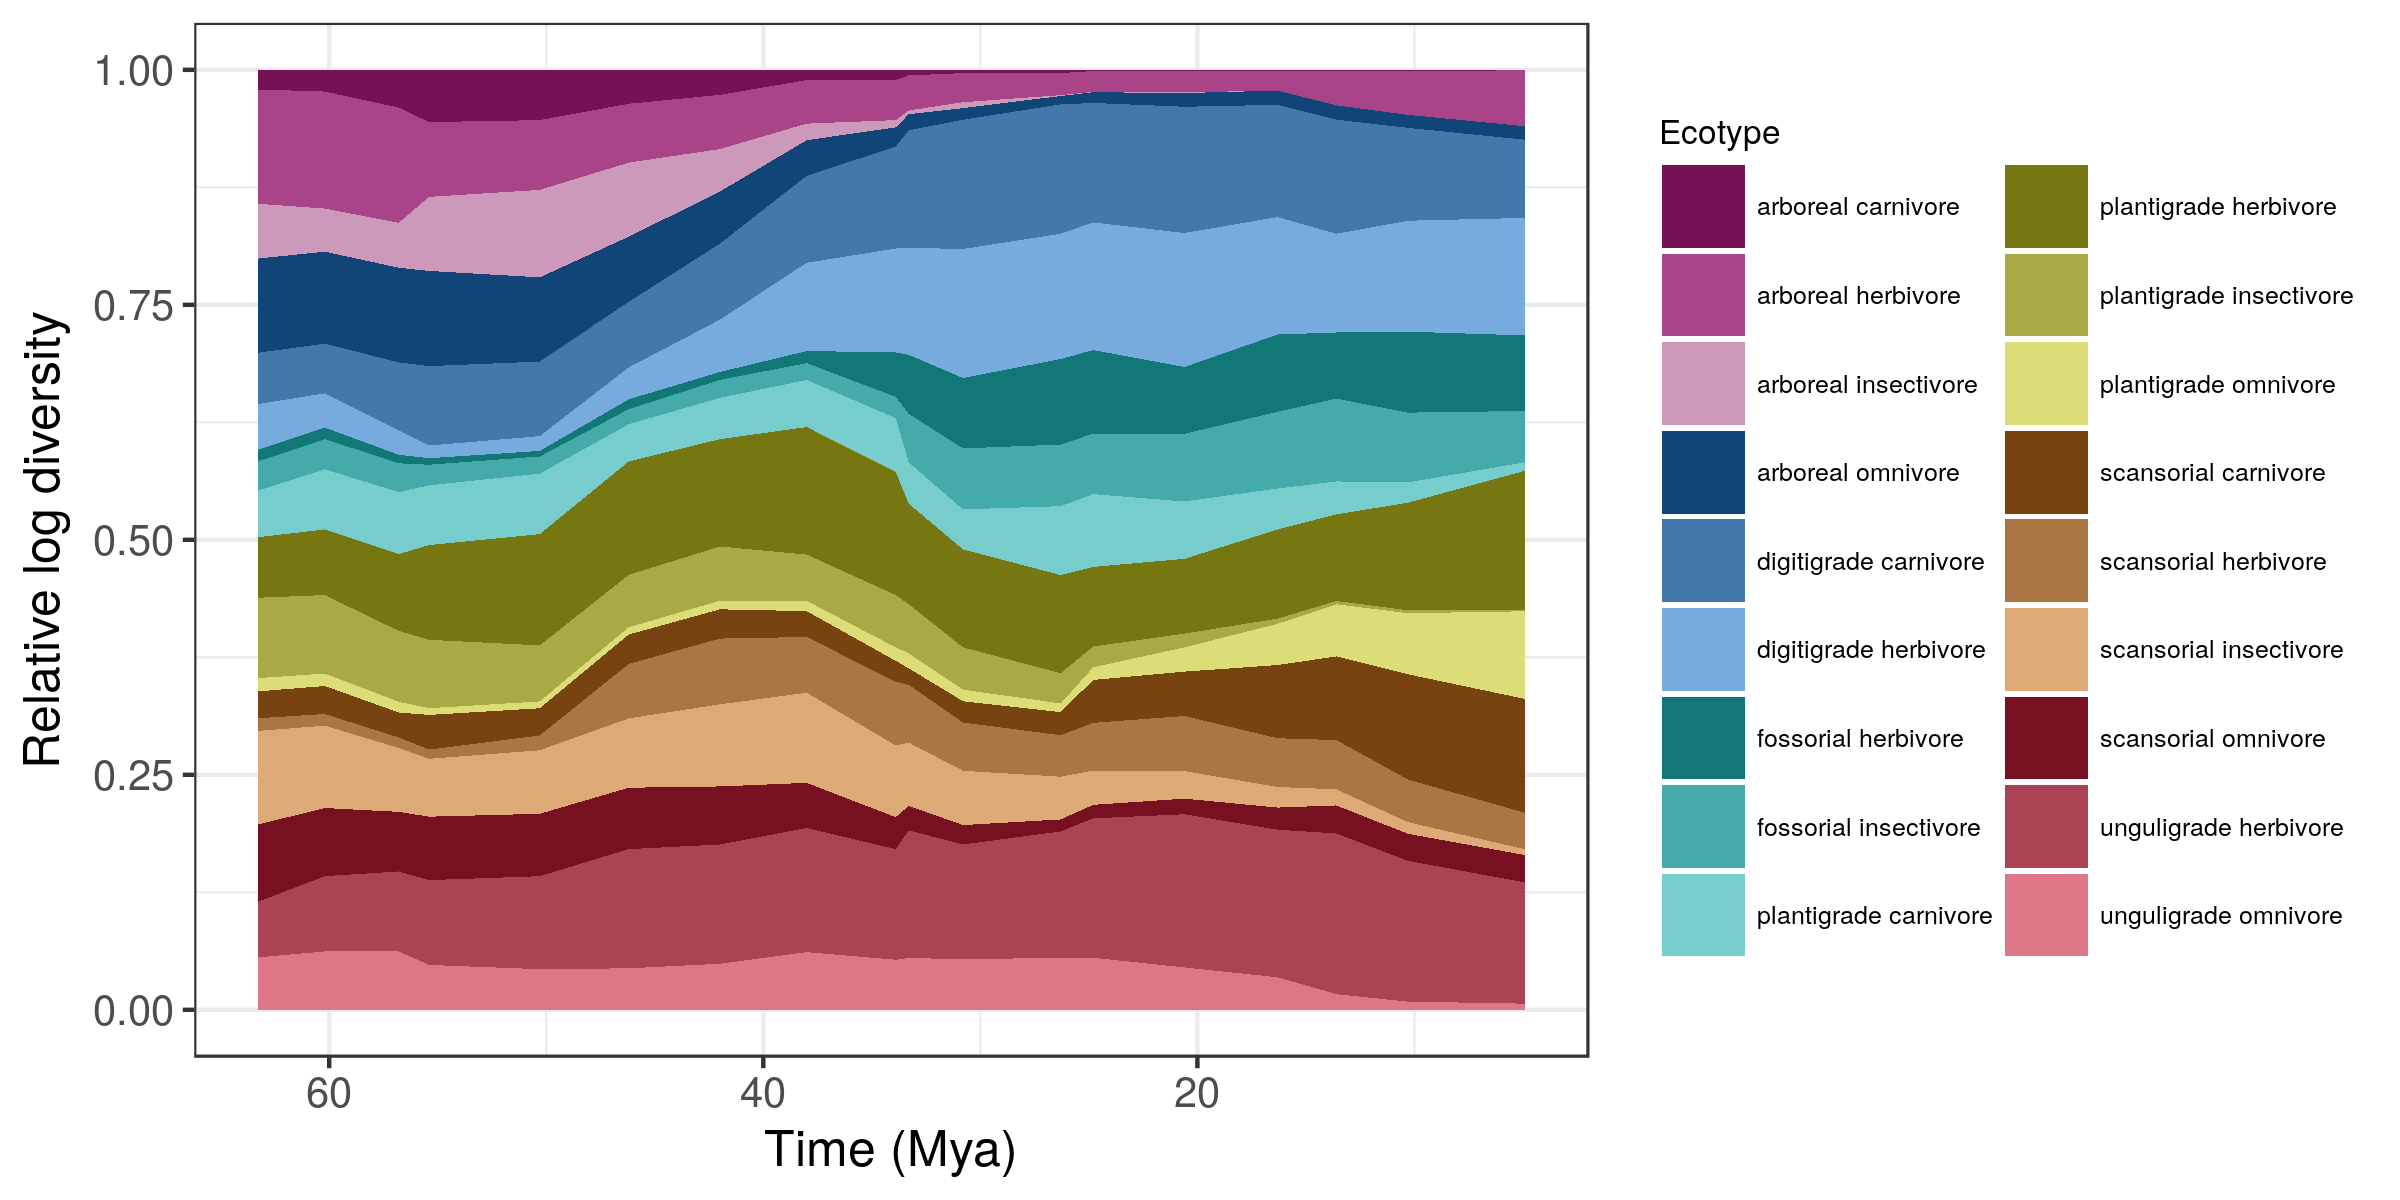
\includegraphics[width=\textwidth,height=0.5\textheight,keepaspectratio=true]{figure/relative_diversity}
  \caption{Relative diversity of the mammal functional groups for the Cenozoic. Relative diveristy was calculated from the mean posterior estimate of standing diversity (Fig. \ref{fig:ecotype_diversity}) and is plotted here without uncertainty. These estimates are calculated from 100 posterior estimates of the true occurrence matrix \(z\) (Table \ref{tab:basic}).}
  \label{fig:ecotype_relative}
\end{figure}


\end{document}

